 %!TEX root = Thesis.tex

\chapter{Coordination Complexes with Rhodium}
\chaptermark{Rhodium}
\label{ch:rhodium}

Rhodium is a very rare element forming only 0.001 ppm of the earth's crust.\cite{Enghag2004Rh}  The majority of the extracted rhodium (81\%) is used in catalytic converters in cars to reduce harmful nitrogen oxides to nitrogen and oxygen.\cite{Heck2001}  Another important use of rhodium is in thermocouples where a rhodium-platinum alloyed wire is used, together with a pure platinum wire for use in high-temperature furnaces.\cite{Enghag2004Rh}  Rhodium coordination complexes form active catalysts, most commonly for hydroformylation and hydrogenation.\cite{Leeuwenbook2000, Cui2005, Pospech2013}  Wilkinson's catalyst, \ce{[RhCl(PPh3)3]}, is one of the most widely known rhodium catalysts, used mainly for the hydrogenation of alkenes, but also for hydroboration of alkenes and selective hydrosilylation of $\alpha$,$\beta$-unsaturated carbonyl compounds.\cite{Osborn1966, Evans1988, Ojima1982}

The 2001 Nobel Prize in Chemistry was awarded to Knowles,\cite{Knowles2002} Noyori,\cite{Noyori2002} and Sharpless\cite{Sharpless2002} for their work in asymmetric catalysis, including several rhodium catalysts.  A derivative of Wilkinson's catalyst, where triphenylphosphine was replaced by the chiral phosphine ($-$)-\ce{PMePh^iPr}, was reported by Knowles and Sabacky in 1968\cite{Knowles1968}.  This chiral version of Wilkinson's catalyst was the first asymmetric hydrogenation catalyst yielding an enantiomeric excess of 15\% when hydrogenating $\alpha$,$\beta$-unsaturated carbonyls (Scheme \ref{Knowlesscheme}).  This was improved by the development of the CAMP ligand (Figure \ref{chiralrhodiumligands}), which gives an enantiomeric excess of 80\% in the hydrogenation of dehydroamino acids, a key step in the commercial production of \iupac{\L-DOPA}, a drug used in the treatment of Parkinson's disease.\cite{Noyori2007}  Rhodium complexes containing chiral diphosphines also form active catalysts, for example a [Rh(\acrshort{cod})\iupac{\cip{S}-BINAP}] (Figure \ref{chiralrhodiumligands}) catalyst is active for the asymmetric isomerisation of allylic amines, a key step in the industrial synthesis of ($-$)-menthol generating over 1000 tons per year.\cite{Noyori2002}

\begin{scheme}[h]
\begin{center}
\vspace{0.5cm}
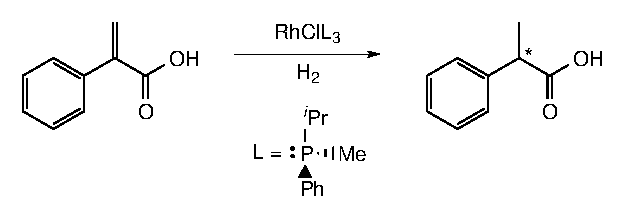
\includegraphics{../Schemes/Knowlesscheme.eps}
\caption[Asymmetric catalytic hydrogenation developed by Knowles]{Asymmetric catalytic hydrogenation developed by Knowles.\cite{Knowles2002}}
\vspace{0.2cm} 
\label{Knowlesscheme}
\end{center}
\end{scheme}
\vspace{0.2cm}

\begin{figure}[h]
\begin{center}
\vspace{0.5cm}
	\begin{subfigure}{0.2\textwidth}
		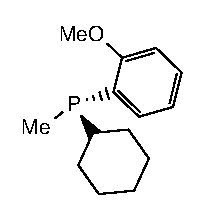
\includegraphics{../Structures/CAMP.eps}
	\end{subfigure}
	~~~~~~~~~~~~~~~~~~
	\begin{subfigure}{0.2\textwidth}
		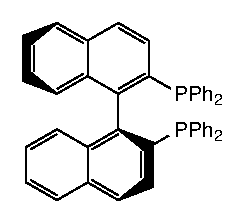
\includegraphics{../Structures/BINAP.eps}
	\end{subfigure}
\caption[Chiral phosphine ligands used in asymmetric catalysis]{Chiral phosphine ligands CAMP (left) and \iupac{\cip{S}-BINAP} (right), used in asymmetric catalysis.\cite{Noyori2007, Noyori2002}}
\vspace{0.2cm}
\label{chiralrhodiumligands}
\end{center}
\end{figure}
\vspace{0.2cm}

%The xantphos class of ligands have long been studied for their role as ancillary ligands in  rhodium catalysed hydroformylation.  

The xantphos class of ligands were first studied for potential use as ancillary ligands in rhodium-catalysed hydroformylation\cite{Kranenburg1995}.  Small changes in the bite-angle can result in changes in reactivity and selectivity.  For hydroformylation the larger bite-angle ligand, \Phxantphos{}, showed a greater selectivity for the linear aldehyde than \Phsixantphos{} or \Phthixantphos{}.  Xantphos ligands have the ability to coordinate to a metal centre in a number of different modes.  The most common is the diphosphine \dento{}\emph{PP\textprime} mode.  Tridentate \POP{} complexes of the xantphos ligands are also relatively common, especially in octahedral complexes.  In this \POP{} coordination mode, the xantphos ligand typically coordinates to the metal in a meridional manner, although facial complexes have also been reported.\cite{Dallanegra2012, Pawley2012}  

Subsequent to the research reported in this chapter being performed, one paper has been published, reporting the coordination chemistry of the \tBuxantphos{} ligand with rhodium.\cite{Haibach2013}  \tBuXantphos{} was shown to react with [Rh(coe)(\hapto{}-Cl\ce{]2} forming a [Rh(\tBuxantphosk)Cl] complex.  This complex readily splits hydrogen to form a [Rh(\tBuxantphosk)Cl(H\ce{)2}] complex.  Both of these complexes were also synthesised as part of the present study and comparison of the results will be discussed where relevant.  Chloride abstraction from  [Rh(\tBuxantphosk)Cl(H\ce{)2}] using \ce{AgBF4} or \ce{AgSbF6} generates the trigonal bipyramidal dihydride complex [Rh(\tBuxantphosk)\ce{(H)2]+}.  This dihydride reacts with ethene to give ethane and [Rh(\tBuxantphosk)\ce{(C2H4)}], however no reaction with the commonly used hydrogen acceptors \emph{t}-butylethylene or norbornene was observed, nor was any reaction with terminal alkenes.  [Rh(\tBuxantphosk)Cl(H\ce{)2}] reacts with \ce{KO^{t}Bu} resulting in a four coordinate mono-hydride species [Rh(\tBuxantphos)H].  [Rh(\tBuxantphos)H] is an active catalyst for the isomerisation of 1-hexene, with a TON of 2000 after 16 hours.  Addition of ethene to this rhodium(I) hydride resulted in the reversible formation of an ethyl complex.  This paper shows some of the interesting chemistry of \tBuxantphos{} with rhodium.  However, to date the coordination chemistry of \tBusixantphos{} and \tButhixantphos{} has not been reported.  

This chapter presents research into the coordination chemistry of \tBusixantphos, \tButhixantphos, and \tBuxantphos{} with rhodium.  The goal was the synthesis and characterisation of complexes that may form as part of catalytic reactions.  As such, this work focusses on the reactivity of a simple rhodium(I) complex towards small molecules, particularly the chemistry towards hydrogen and carbon monoxide, as these are common components of catalytic systems.  

\section{Synthesis of [Rh(\POP)Cl] Complexes}
\label{section:rhodiumchloride}

Chlorido-bridged rhodium alkene dimers are commonly used starting materials for the formation of rhodium phosphine complexes.  These dimers can react in a number of different ways depending on the phosphine ligand used (Figure \ref{RhcoeClcomplexes}).  When two equivalents of a monophosphine react with [Rh(\acrshort{coe}\ce{)2Cl]2}, (\acrshort{coe} = \acrlong{coe}) the phosphine displaces one \acrshort{coe} molecule from each rhodium forming a symmetric dimer.\cite{Canepa2003}  These complexes are typically unstable.  Further addition of phosphine displaces the remaining two \acrshort{coe} molecules, while retaining the chlorido-bridged rhodium core.\cite{Bleeke1986}  Analogous complexes form when the reaction is carried out with diphosphines.\cite{Fryzuk1989}  In some cases, bidentate ligands can cleave the dimer resulting in a [Rh(LL)(\acrshort{coe})Cl] complex.\cite{Hashimoto2010}  Tridentate ligands are also able to cleave the dimer and result in the mononuclear complexes \ce{[Rh(LLL)Cl]}\cite{Khan1988, Hermann2002}.  With negatively charged tridentate ligands, a trigonal bipyramidal hydride chloride complex is formed (where the hydride forms \emph{via} X-H activation of the central ligating atom).\cite{Boom1998, Winter2003, Salem2008}  Alternatively, the ligand can be reacted first with a strong base or a silver salt to remove the chloride and break the dimer.  In this case the remaining coordination site is occupied either by the anion from the silver salt, or by a cyclooctene molecule if a non-coordinating counterion is used.\cite{Fryzuk1986, Hanson2008}

\begin{figure}[h!]
\begin{center}
\vspace{0.5cm}
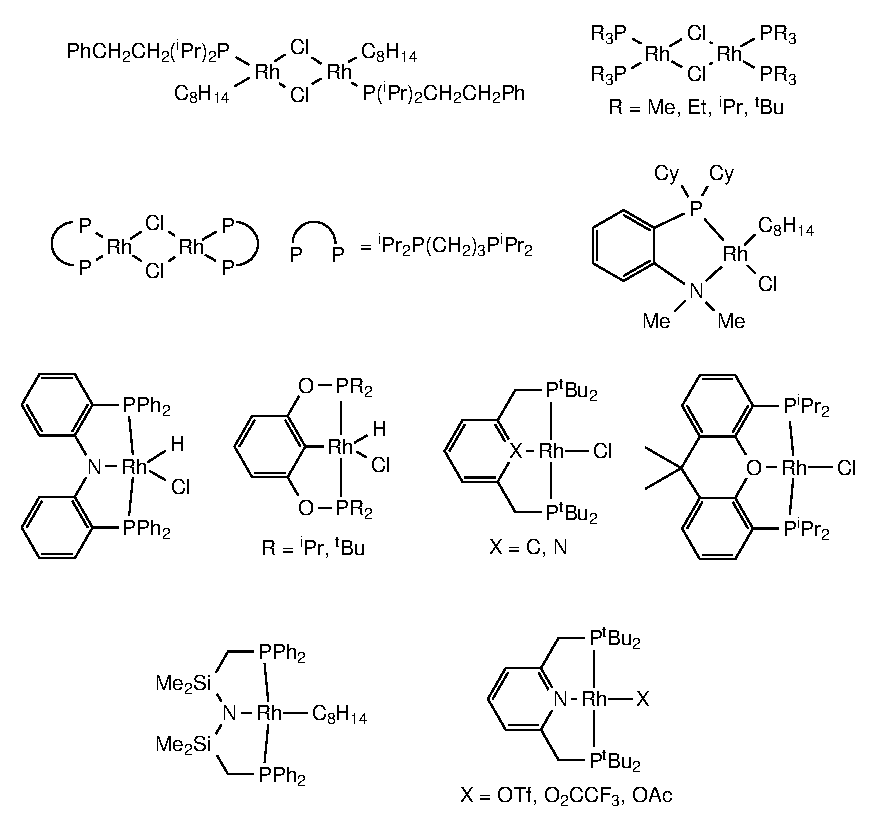
\includegraphics{../Figures/RhCOEClcomplexes.eps}
\caption[Complexes from \ce{[Rh(coe)2Cl]2} and phosphine ligands]{Complexes formed by reaction of \ce{[Rh(coe)2Cl]2} and phosphine ligands.  First row: monophosphines in 2:1 and 4:1 ligand:\ce{[Rh(coe)2Cl]2}, second row: bidentate ligands, third row: tridentate ligands in the absence of other reagents, fourth row: tridentate ligands using lithiated ligand (left) or a silver salt (right).}
\vspace{0.2cm}
\label{RhcoeClcomplexes}
\end{center}
\end{figure}
\vspace{0.2cm}

Reaction between [Rh(\acrshort{coe}\ce{)2Cl]2} and the three \tBuxantphos{} ligands was carried out on an NMR scale in \ce{C6D6}.  No reaction occurred at room temperature overnight except in the case of \tBuxantphos{}, which displays a small amount of conversion, evident from the \proton{} and \phosphorus{} NMR spectra.  The lack of reactivity at room temperature may be the result of the poor solubility of [Rh(\acrshort{coe}\ce{)2Cl]2} in \ce{C6D6}.  Upon heating to 60 \degC{} coordination of the \tBuxantphos{} ligands proceeded, going to completion after 24 hours.  For all three \tBuxantphos{} ligands the product is the expected [Rh(\tBuxantphosk)Cl] mononuclear complex (Scheme \ref{RhodiumI}).  This complex is directly analogous to an \iPrxantphos{} complex reported in 2013\cite{Esteruelas2013}, which was synthesised in the same manner.  The \tBuxantphos{} ligands have a number of different possible coordination modes.  In this case a meridional \POP{} pincer coordination is observed.  It is likely that the reaction proceeds by substitution of one cyclooctene ligand with one of the phosphorus atoms, followed by a second to form a chlorido-bridged dimer.  However, as the \tBuxantphos{} ligands have such large bite-angles and the potentially coordinating ether bridge, this can readily split the dimer resulting in the desired product.  None of these intermediates were observed, indicating low activation barriers once the first substitution had occurred.

\begin{scheme}[htb]
\begin{center}
\vspace{0.5cm}
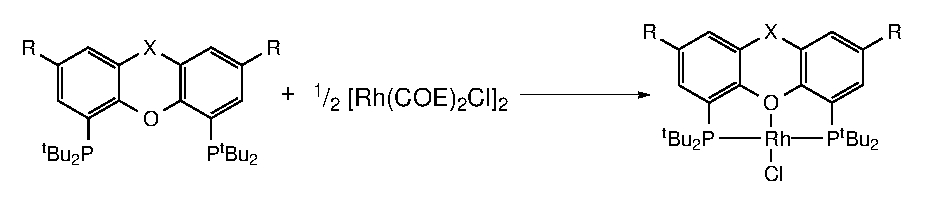
\includegraphics{../Schemes/RhodiumI.eps}
\caption[Reaction of \ce{[Rh(coe)2Cl]2} and \tBuxantphos{} ligands]{Reaction of \ce{[Rh(coe)2Cl]2} and \tBuxantphos{} ligands.  \emph{Reagents and conditions:} (i) \ce{0.5 eq. [Rh(\acrshort{coe}\ce{)2Cl]2}}, \ce{C6D6}, 60\degC, 24 hours.}
\vspace{0.2cm} 
\label{RhodiumI}
\end{center}
\end{scheme}
\vspace{0.2cm}

% taken out from the scheme caption \tBuxantphos: R = H, X = \ce{CMe2}. \tButhixantphos: R = Me, X = S. \tBusixantphos: R = H, X = \ce{SiMe2}

The \proton{}, \carbon{} and \phosphorus{} NMR spectra for the three [Rh(\tBuxantphosk)Cl] complexes are consistent with the proposed structures.  Representative \proton{} and \phosphorus{} NMR spectra for [Rh(\tBuxantphos)Cl] are shown in Figure \ref{RhClnmr} and selected NMR data for all three complexes is given in Table \ref{table:rhodiumchloride}.  In the \phosphorus{} NMR spectra the signals shift downfield by 35.8--37.5 ppm upon coordination, with the peaks for the complexes appearing at 44.2--47.7 ppm.  The signals for the complexes are doublets with rhodium coupling of 140.0--142.3 Hz.  This coupling is consistent with a rhodium(I) complex and is similar to the coupling constant for [Rh(\iPrxantphosk)Cl] (142.4 Hz).\cite{Esteruelas2013}  The \proton{} and \carbon{} NMR spectra support the proposed structure, as the \tBu{} proton and carbon signals all appear as virtual triplets, indicating strongly coupled phosphorus atoms, which typically occurs in a \trans{} coordination geometry.\cite{Harris1964, Pregosin2012}  In the \carbon{} NMR spectrum the peak corresponding to the \emph{O}-\emph{ipso} carbon has shifted downfield relative to the free ligand, unlike the equivalent [Ag(\tBuxantphos)Cl] complexes where the oxygen is known to be non-coordinating (Table \ref{table:oxygenbindingrh}).  This downfield shift is consistent with a coordinated oxygen.  As the oxygen donates electron density to the metal this will inductively decrease electron density on the \emph{O}-\emph{ipso} carbon resulting in decreased shielding and thus a downfield shift of the NMR signal.  %The coupling on the O-ipso carbon decreases from the free ligand to a \dento{2}-\emph{PP\textprime} complex, but increases in the [Rh(\tBuxantphosk)Cl] complexes.  \fixme{why}

\begin{figure}[htbp]
\begin{center}
\vspace{0.5cm}
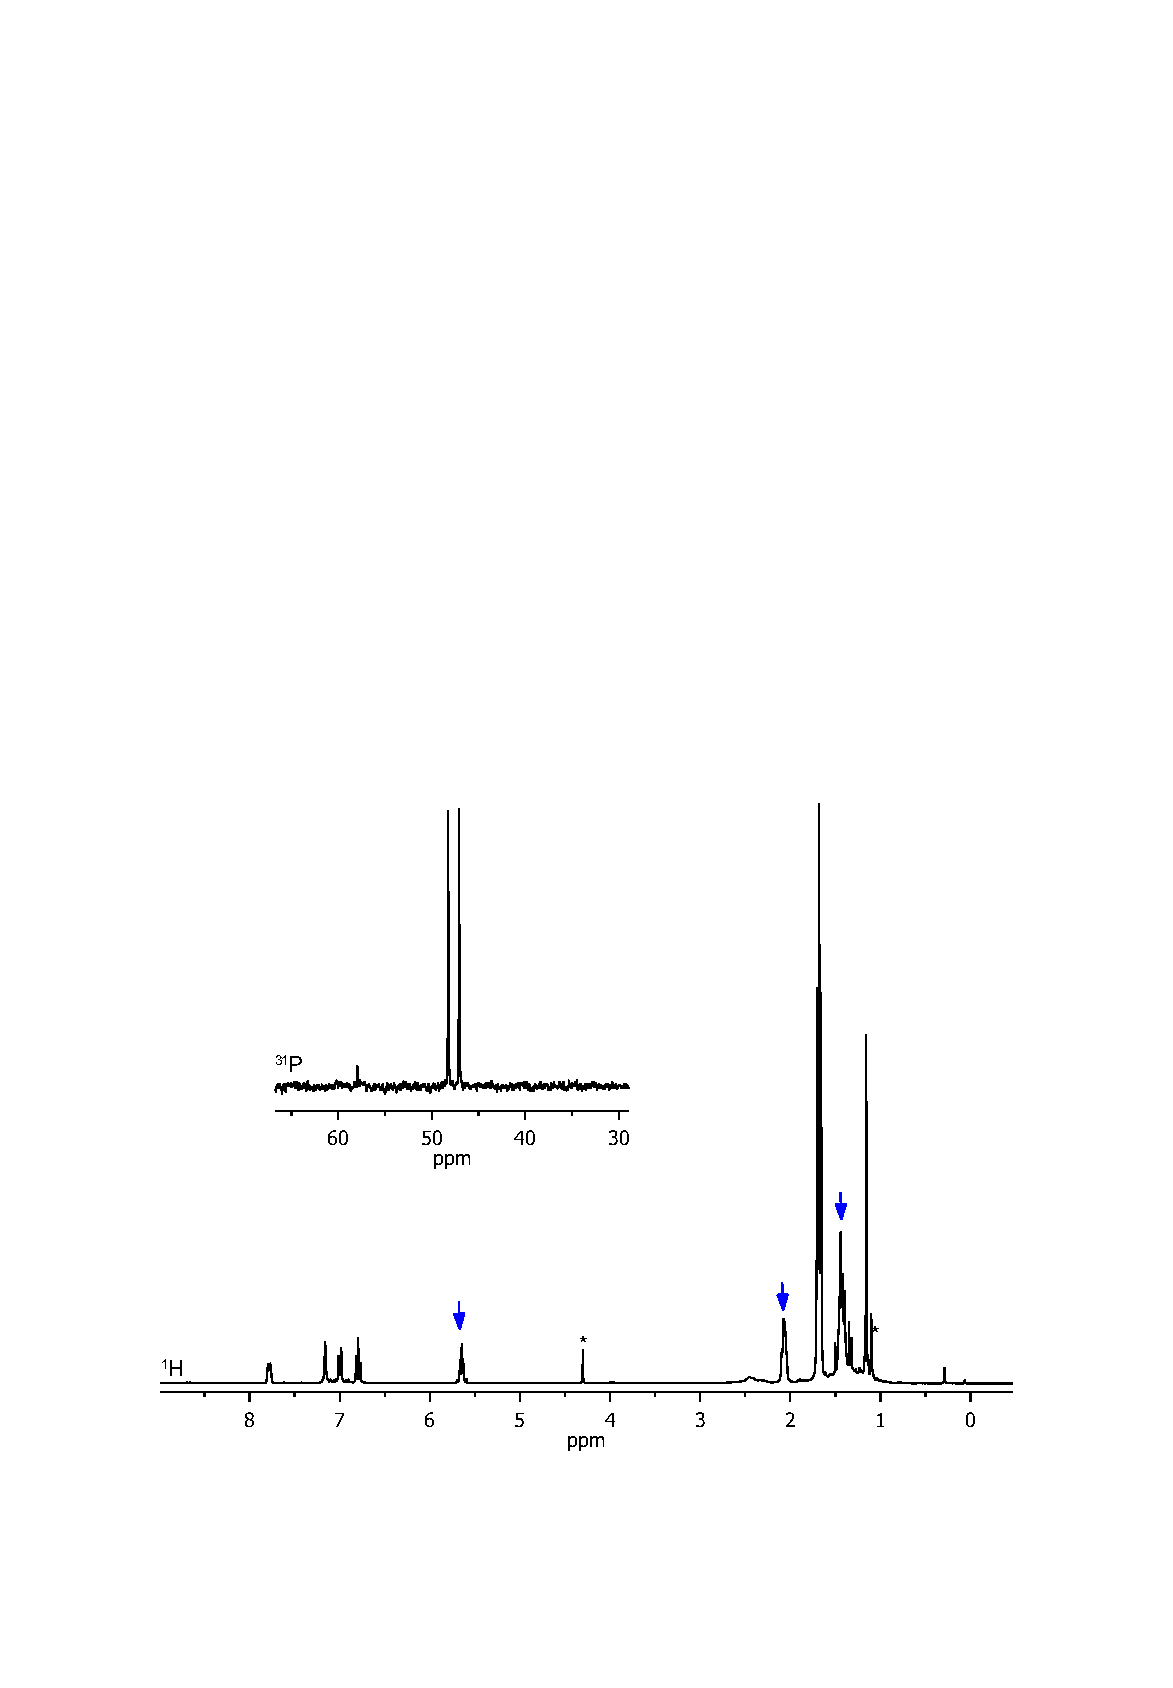
\includegraphics[trim = 2.5cm 4.0cm 2.5cm 15cm, clip]{../NMR/7004B.eps}
\caption[\phosphorus{} and \proton{} NMR spectra for [Rh(\tBuxantphos)Cl{]}]{\phosphorus{} and \proton{} NMR spectra for [Rh(\tBuxantphos)Cl].  Blue arrows indicate displaced \acrshort{coe}, asterisks denote impurities.}
\vspace{0.2cm}
\label{RhClnmr}
\end{center}
\end{figure}
\vspace{0.2cm}

\begin{table}[htbp]
\caption[Selected NMR data of [Rh(\tBuxantphos)Cl{]} complexes]{Selected NMR data of [Rh(\tBuxantphos)Cl] complexes in \ce{C6D6}.}
\vspace{1em}
\label{table:rhodiumchloride}
\small
\begin{center}
\begin{tabular}{c c c c c c}
	\toprule{}
	~ & \multicolumn{3}{c}{\bfseries{\phosphorus}} & \multicolumn{2}{c}{\bfseries{\proton{} \emph{t}-Bu}}\\
	\cmidrule(lr){2-4} \cmidrule(lr){5-6} 
	\bfseries{Compound}&\bfseries{$\delta/$ppm}&\bfseries{$\Delta\delta/$ppm}&\bfseries{\JRhP{}$/$Hz}&\bfseries{$\delta/$ppm}&\bfseries{\J $/$Hz}\\
	\midrule{}
	\tBuSixantphos		&	44.2	&	35.8	&	140.0	& 1.69	& 13.5\\
	\tBuThixantphos	& 	46.5	&	37.0	&	141.5	& 1.67	& 13.7\\
	\tBuXantphos		&	47.7	&	37.5	&	142.3	& 1.68	& 13.4\\
	\bottomrule{}
\end{tabular}
\end{center}
\end{table}

\begin{sidewaystable}[htbp]
\caption[\carbon{} Chemical shift and coupling of the \emph{O}-\emph{ipso} carbon when in the free ligand, [Ag(\tBuxantphos)Cl{]} and [Rh(\tBuxantphos)Cl{]} complexes]{\carbon{} Chemical shift and coupling of the \emph{O}-\emph{ipso} carbon in the free ligand, [Ag(\tBuxantphos)Cl] (\ce{CDCl3}) and [Rh(\tBuxantphos)Cl] (\ce{C6D6}) complexes. $\Delta\delta$ values are $\delta$ complexed - $\delta$ uncoordinated.}
\vspace{1em}
\label{table:oxygenbindingrh}
\small
\begin{center}
\begin{tabular}{l c c c c c c}
	\toprule{}
	~&\bfseries{Ligand (\ce{CDCl3})} &\bfseries{Ligand (\ce{C6D6})} &\multicolumn{2}{c}{\bfseries{[Ag(\tBuxantphos)Cl]}}&\multicolumn{2}{c}{\bfseries{[Rh(\tBuxantphos)Cl]}}\\
	\cmidrule(lr){2-3} \cmidrule(lr){4-5} \cmidrule(lr){6-7}
	\bfseries{Ligand}&\bfseries{$\delta/$ppm}&\bfseries{$\delta/$ppm}&\bfseries{$\delta/$ppm}&\bfseries{$\Delta\delta$}&\bfseries{$\delta/$ppm}&\bfseries{$\Delta\delta$}\\
	\midrule{}
	\tBuSixantphos	&	164.3	& 164.5	&	163.9	& -0.4	& 169.5	& 5.0  \\
	\tBuThixantphos&	155.3	& 155.9	&	155.5	& 0.2 	& 157.4	& 1.5 \\
	\tBuXantphos	&	155.8	& 156.0	&	156.5	& 0.7		& 158.9	& 2.9 \\
	\bottomrule{}
\end{tabular}
\end{center}
\end{sidewaystable}

Subsequent to this work the [Rh(\tBuxantphosk)Cl] complex and X-ray crystal structure has been reported in the literature.\cite{Haibach2013}  The literature method also used [Rh(\acrshort{coe}\ce{)2Cl]2} as the starting material in benzene however, their reaction was complete in 24 hours at room temperature, which may suggesting that the heating to 60 \degC{} is unnecessary.  The NMR data reported herein is consistent with the literature values.  The X-ray crystal structure of [Rh(\tBuxantphosk)Cl] (Figure \ref{crystal:RhCl}) shows a square-planar geometry with a \tBuxantphosk{} coordination mode.  

\begin{figure}[htbp]
\begin{center}
\vspace{0.5cm}
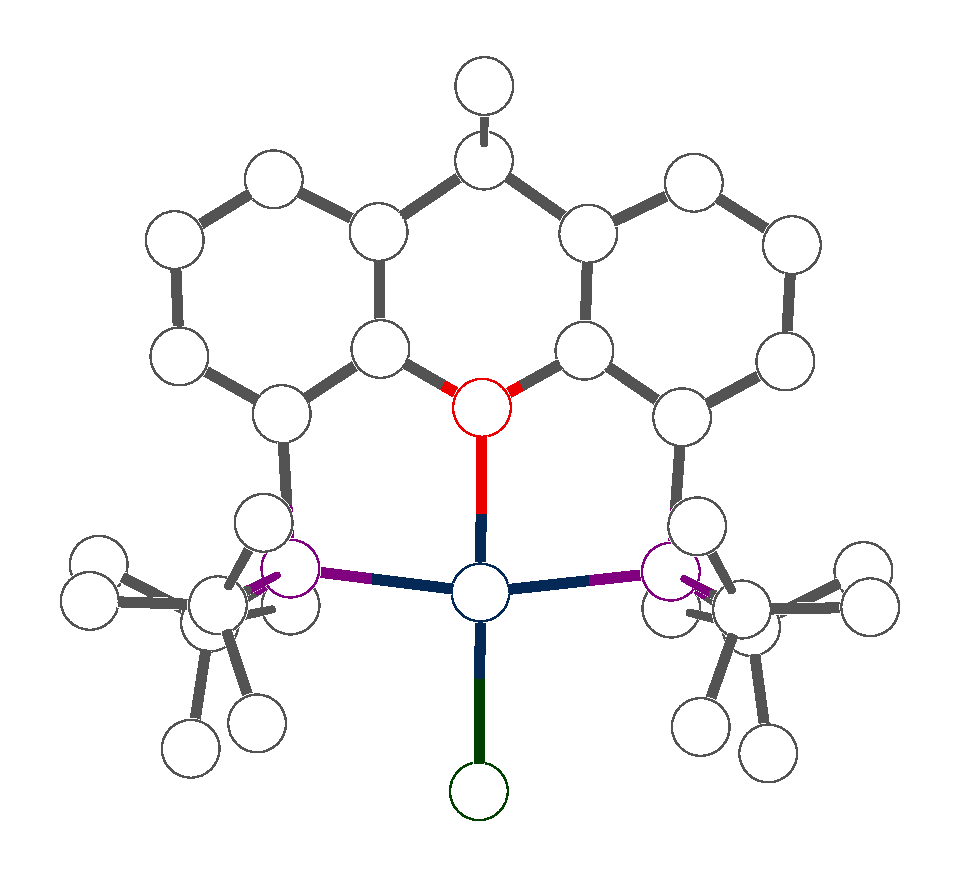
\includegraphics[width=0.5\textwidth]{../Othercrystals/RhCtBuCl.eps}
\caption[X-ray crystal structure of [Rh(\tBuxantphosk)Cl{]}]{X-ray crystal structure of [Rh(\tBuxantphosk)Cl].  Hydrogen atoms omitted for clarity.\cite{Haibach2013}}
\vspace{0.2cm}
\label{crystal:RhCl}
\end{center}
\end{figure}
\vspace{0.2cm}

%A reaction occurs rapidly with all three diphosphine to form complexes \fixme{compound reference} (Scheme \ref{RhodiumI}).  These complexes have \JRhP{} coupling constants of around 142 Hz, consistent with rhodium(I).  The complexes are direct analogues of those reported for \iPrxantphos{} which has a \JRhP{} coupling constant of 142.4 Hz.\cite{Esteruelas2013}  The \tBuxantphos ligands are coordinated in a tridentate manner with the oxygen binding.  In the \carbon{} NMR spectrum this can be seen as the O-ipso carbon carbon has shifted to downfield.  For example in \tBuxantphos{} this carbon resonants at 155.8 ppm, in the complex \ce{[(tBu-xantphos)AgCl]} the carbon shifted to 156.5 although the oxygen was not binding.  In the tridentate rhodium complex this carbon has moved downfield again to 158.9 ppm.  This shift in the resonant frequency of this carbon is a result of the oxygen donating electron density to the rhodium, which in turn makes the oxygen withdraw electron density from the ipso carbons.  

\section{Reaction with Hydrogen}
\label{section:rhodiumhydride}

Rhodium complexes are well-known as homogeneous hydrogenation and hydroformylation catalysts.  Both of these processes involve the activation of molecular hydrogen at the rhodium centre.  The catalytic cycle for hydrogenation using monophosphine ligands (Scheme \ref{Hydrogenationcycle}) involves the addition of molecular hydrogen to \ce{[Rh(PR3)2Cl]} generating a rhodium dihydride, which then coordinates an alkene and undergoes hydride-migration followed by reductive elimination to generate the starting rhodium complex and the alkane. In hydroformylation (Scheme \ref{Hydroformylationcycle}) the alkene coordinates to an existing rhodium hydride complex.  Hydride migration, occurs followed by carbon monoxide coordination and migratory insertion into the rhodium alkyl bond.  This is followed by the oxidative addition of dihydrogen, generating a rhodium(III) dihydride complex.  The cycle concludes by reductive elimination, generating the aldehyde and the starting rhodium(I) complex.  The influence of the bite-angle of \Phxantphos{} complexes on the reactivity and selectivity of catalytic process was first studied for hydroformylation.\cite{Kranenburg1995}  Since then hydroformylation has been studied extensively using a variety of xantphos derivatives.\cite{Bronger2002, Bronger2003, Bronger2004, Bronger2004b, Bronger2004c, Buhling1997, Buhling1997b, Dieleman2001, Dierkes1999, Freixa2003, Goedheijt1998b, Kamer2001, Leclercq2005, Leeuwen1999, Leeuwen2000, Mora2007, Sandee1999, Silva2003, Veen1999, Veen2000, Vlugt2004, Zuidema2007, Zuidema2008, Zuidema2010}  Given the importance of the oxidative addition of molecular hydrogen for both hydrogenation and hydroformylation, and to investigate any possible differences of the wide bite-angle and steric bulk of the \tBuxantphos{}, ligands we investigated the reactivity of the [Rh(\tBuxantphosk)Cl] complexes with dihydrogen.  

\begin{scheme}[htbp]
\begin{center}
\vspace{0.5cm}
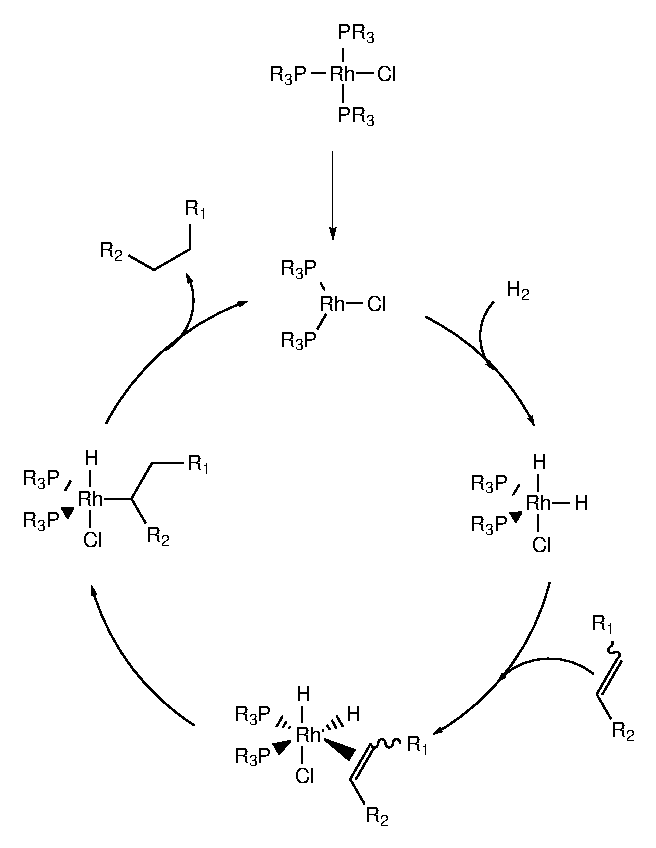
\includegraphics{../Schemes/Homogeneoushydrogenation.eps}
\caption[Catalytic cycle for homogeneous hydrogenation]{Catalytic cycle for homogeneous hydrogenation using a rhodium chloride complex with monophosphine ligands.}
\vspace{0.2cm}
\label{Hydrogenationcycle}
\end{center}
\end{scheme}

\begin{scheme}[htbp]
\begin{center}
\vspace{0.5cm}
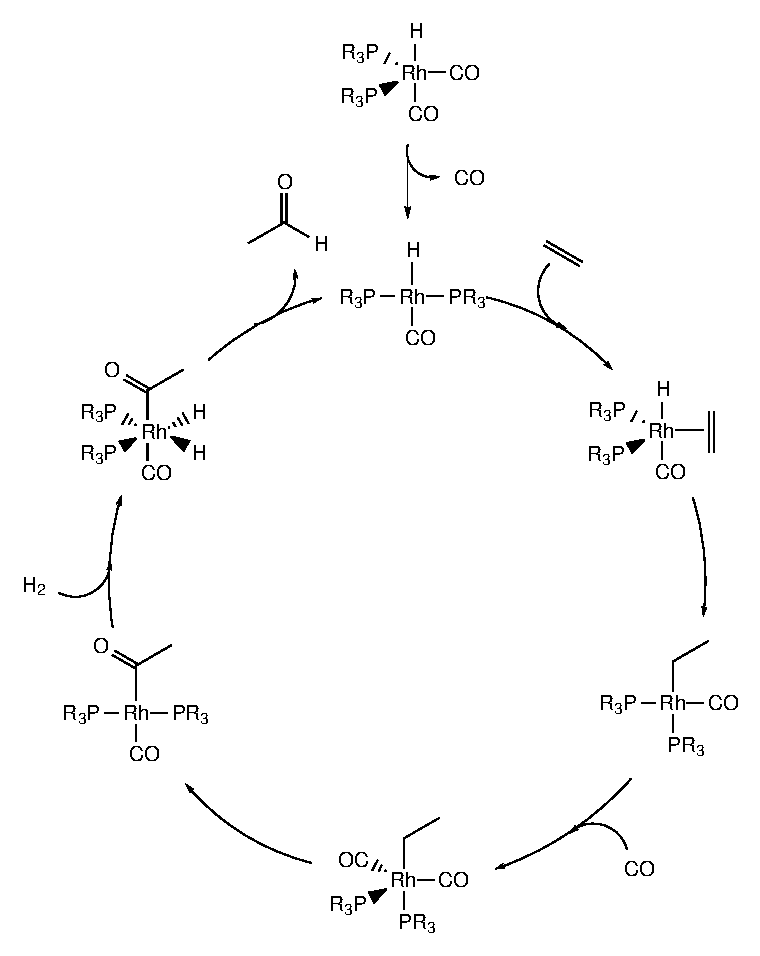
\includegraphics{../Schemes/Hydroformylationcycle.eps}
\caption[Catalytic cycle for homogeneous hydroformylation]{Generic catalytic cycle for homogeneous hydroformylation.}
\vspace{0.2cm}
\label{Hydroformylationcycle}
\end{center}
\end{scheme}

%%%%%%%%\fixme{Kathryn had changes for these structures}

The [Rh(\tBuxantphosk)Cl] complexes react readily with hydrogen, forming octahedral rhodium(III) dihydride complexes (Scheme \ref{Rhodiumhydride}).  The dihydrogen is split forming two classical hydride ligands with a \cis{} configuration.  The \tBuxantphos{} ligands retain their meridional coordination, meaning that the hydride ligands are in different environments, one \trans{} to the chloride and the other \trans{} to the oxygen donor atom.  As a result, the two faces of the \tBuxantphos{} ligands are now different causing two different environments for the bridgehead methyls in both \tBusixantphos{} and \tBuxantphos{}, and the \tBu{} groups for all three \tBuxantphos{} ligands.  However, the plane of symmetry perpendicular to the \tBuxantphos{} backbone is retained, such that the methyl substituents of \tButhixantphos{} are in the same environment.  

\begin{scheme}[htbp]
\begin{center}
\vspace{0.5cm}
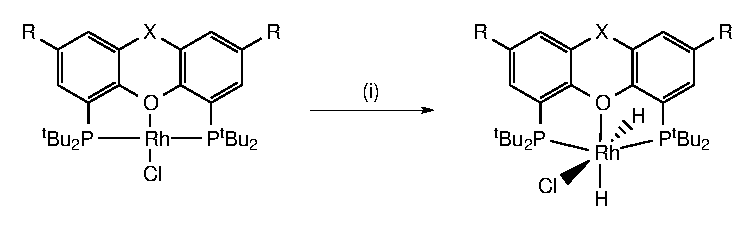
\includegraphics{../Schemes/Rhodiumhydride.eps}
\caption[Reaction of [Rh(\tBuxantphos)Cl{]} with hydrogen]{Reaction of the Rh(\tBuxantphos)Cl] complexes with hydrogen. \emph{Reagents and conditions:} (i) \ce{H2}, \ce{C6D6}.}
\vspace{0.2cm} 
\label{Rhodiumhydride}
\end{center}
\end{scheme}
\vspace{0.2cm}

%tBu-xantphos: R = H, X = \ce{CMe2}. tBu-thixantphos: R = Me, X = S. tBu-sixantphos: R = H, X = \ce{SiMe2}}

Two hydride resonances are evident in the \proton{} NMR spectra of the three [Rh(\tBuxantphosk)Cl\ce{(H)2}] complexes.  The signals appear upfield as well defined doublets of triplets of doublets, coupling to the rhodium, two phosphorus atoms and each other (Figure \ref{rhodiumhydridenmr}, Table \ref{table:dihydrides}).  The hydride \emph{trans} to the chloride ligand (-16.92 to -17.04 ppm) shows very little difference in either the chemical shift or coupling constants between the three complexes.  The hydride \trans{} to the \tBuxantphos{} oxygen (-20.51 to -21.12 ppm) shows more variation in the chemical shift and coupling.  The value of \JRhH{} decreases with increasing natural bite-angle, such that the \tBuxantphos{} complex has the lowest value and \tBusixantphos{} the largest.  This
suggests that the \trans{} influence of the ether bridge is highest for \tBuxantphos{} and lowest for \tBusixantphos, which may be related to the amount of strain required for the ligand to achieve tridentate coordination.  

% indicates that the \trans{} influenceAs the bite-angle for the \tBuxantphos{} ligand increases, the ligand will require less energy to adopt a pincer coordination mode.  

%Thereby, the \trans{} influence of the ether donor will be related to the bite-angle of the ligand 

%This results in the larger bite-angle ligands adopting a mode closer to the ideal T-shaped pincer coordination causing a smaller Rh-O bond length.  This stronger bond in the \trans{} position results in a decreased coupling constant for the hydride ligand.  

\begin{figure}[htbp]
\begin{center}
\vspace{0.5cm}
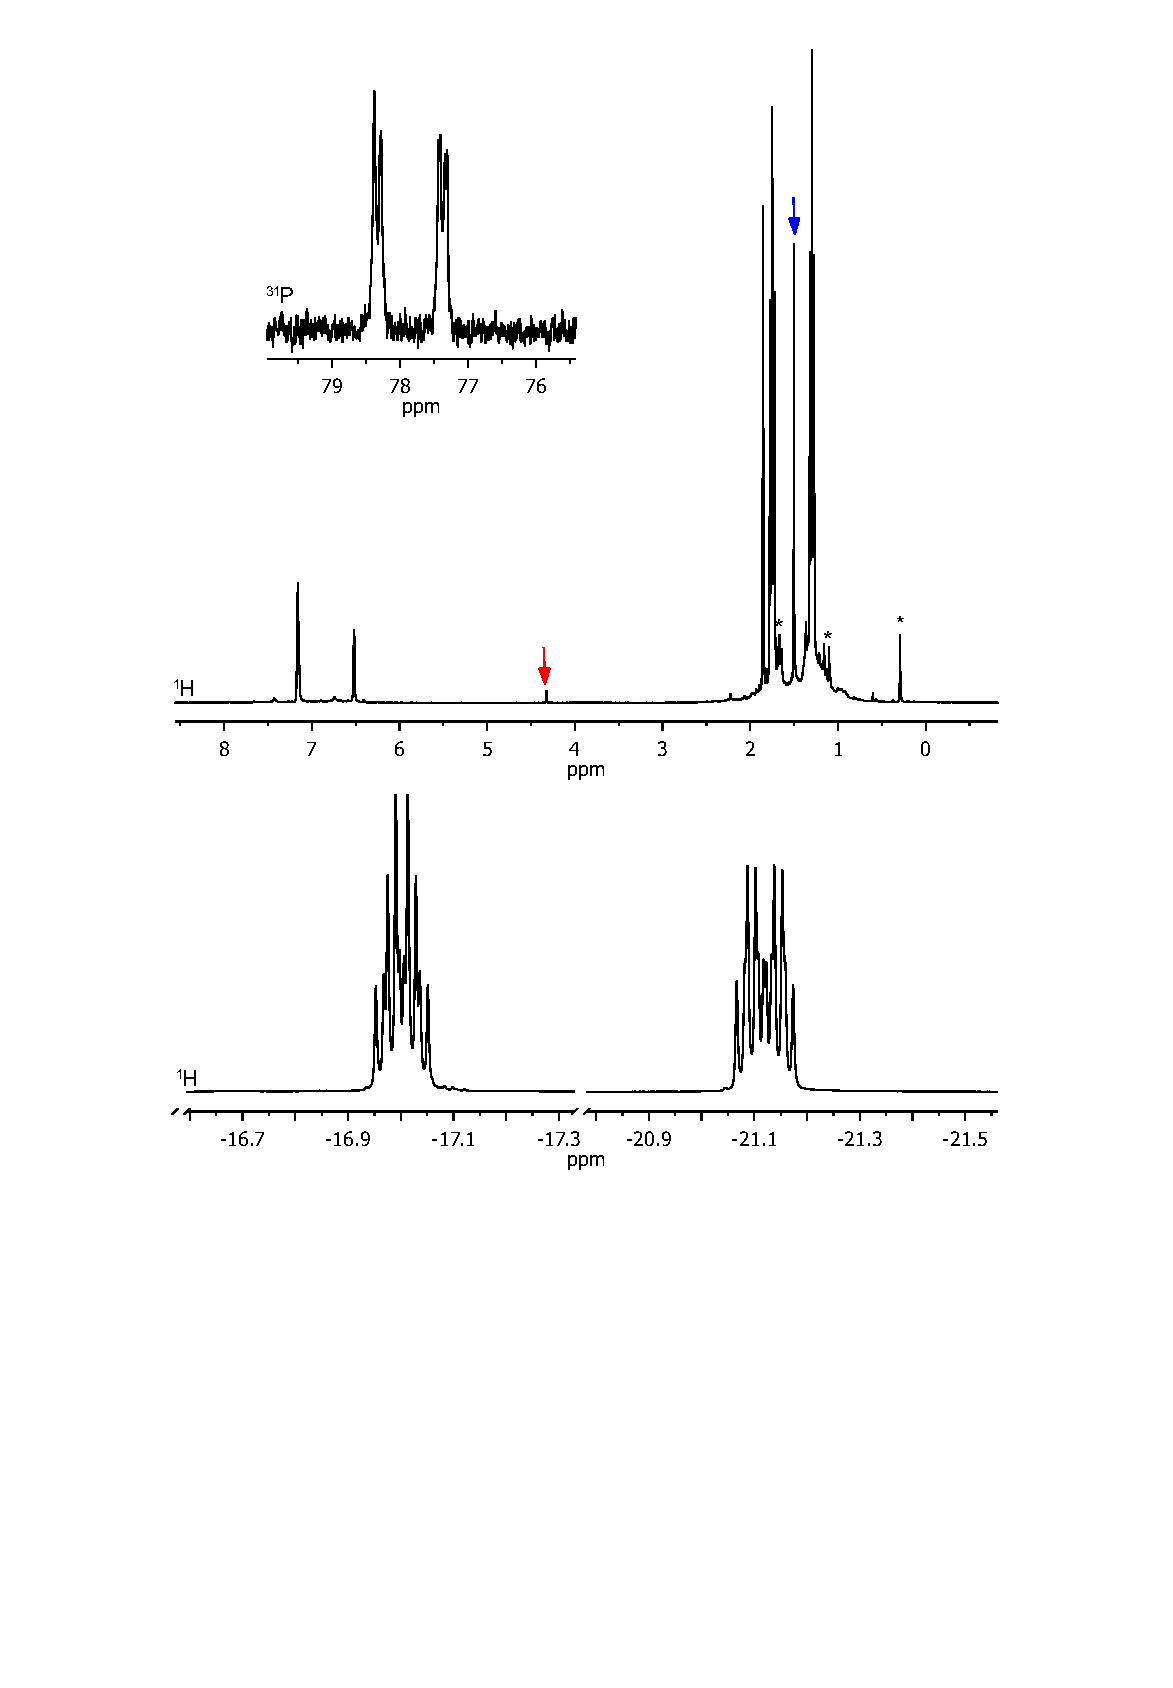
\includegraphics[trim = 2.5cm 8.5cm 2.5cm 0cm, clip]{../NMR/7006E.eps}
\caption[NMR spectra for [Rh(\tButhixantphos)\ce{Cl(H)2]}]{NMR spectra for \texorpdfstring{[Rh(\tButhixantphos)\ce{Cl(H)2]}} R in \ce{C6D6}.  Impurities are indicated by asterisks, \ce{CH2Cl2} is indicated by a red arrow and cyclooctane by a blue arrow.}
\vspace{0.2cm}
\label{rhodiumhydridenmr}
\end{center}
\end{figure}
\vspace{0.2cm}

\begin{sidewaystable}
\caption[Hydride \proton{} NMR data for [Rh(\tBuxantphosk)Cl(\ce{H)2]}]{Hydride \proton{} NMR data for \texorpdfstring{Rh(\tBuxantphosk)Cl(H\ce{)2]}}R complexes in \ce{C6D6}.}
\vspace{1em}
\label{table:dihydrides}
\small
\begin{center}
\begin{tabular}{c c c c c c c c c}
\toprule{}
	~~ & \multicolumn{4}{c}{\bfseries{\ce{H-} \trans-\ce{Cl-}}} & \multicolumn{4}{c}{\bfseries{\ce{H-} \trans-O}}\\
	\cmidrule(lr){2-5} \cmidrule(lr){6-9} 
	\bfseries{Diphosphine}&\bfseries{$\delta/$ppm}&\bfseries{\JRhH$/$Hz}&\bfseries{\JPH$/$Hz}&\bfseries{\JHH$/$Hz}&\bfseries{$\delta/$ppm}&\bfseries{\JRhH$/$Hz}&\bfseries{\JPH$/$Hz}&\bfseries{\JHH$/$Hz}\\
	\midrule{}
	\tBuSixantphos & -16.92 & 22.7 & 13.5 & 9.4 & -21.12 & 30.9 & 12.1 & 9.2 \\
	\tBuThixantphos & -17.00 & 22.6 & 13.5 & 9.4 & -21.13 & 30.5 & 12.4 & 9.4 \\
	\tBuXantphos & -17.04 & 22.8 & 13.4 & 9.4 & -20.51 & 28.8 & 12.2 & 9.4 \\
	\bottomrule{}
\end{tabular}
\end{center} 
\end{sidewaystable}

The \phosphorus{} NMR spectra (example in Figure \ref{rhodiumhydridenmr} for \tButhixantphos) for the [Rh(\tBuxantphosk)Cl\ce{(H)2]} complexes each display a single resonance, downfield relative to the starting [Rh(\tBuxantphosk)Cl] complexes, as a doublet of doublets with some further coupling evident.  Although \phosphorus{} NMR is \proton{} decoupled, the decoupler is sometimes unable to fully decouple resonances that are so far outside the typical \proton{} NMR range (-2 to 15 ppm) resulting in residual coupling.  The values of \JRhP{} in the [Rh(\tBuxantphosk)Cl\ce{(H)2]} complexes are 116.1--117.8 Hz, a decrease of 23.7--25.3 Hz from the starting [Rh(\tBuxantphosk)Cl] complexes.  This decrease is consistent with a change in the oxidation state from rhodium(I) to rhodium(III).\cite{Pregosin2012} Two signals are observed in the \proton{} NMR spectra for the \tBu{} protons in all three complexes consistent with the proposed geometry.  Both signals are virtual triplets, confirming the mutually \trans{} coordination of the phosphorus atoms, consistent with the proposed meridional coordination of the ligands.  Two signals were also observed in the \proton{} NMR spectra for the bridgehead methyls in [Rh(\tBuxantphosk\ce{)Cl(H)2]} and [Rh(\tBusixantphosk\ce{)Cl(H)2]}, again consistent with the proposed structure.  

The [Rh(\tBuxantphosk\ce{)Cl(H)2]} complexes are similar to previously reported rhodium xantphos dihydride complexes,  [Rh\ce{(H)2}(\iPrxantphos)X] (X = Cl, OTf)\cite{Esteruelas2013} and [Rh\ce{(H)2}(\Phxantphos)X\ce{]+} (X = P(\acrshort{Cyp}\ce{)3} \acrshort{Cyp} = \acrlong{Cyp}, NCMe, \ce{OC(Me3)2}, \ce{H3BNMe3}-\dento{}\emph{H})\cite{Dallanegra2012, Johnson2013, Pawley2010}.   In these cases the hydride \trans{} to the oxygen atom was located in the \proton{} NMR between -22.19 and -19.00 ppm with a rhodium coupling constant of 27.0--33.8 Hz.  The \proton{} NMR signals for the hydride ligands in the [Rh(\tBuxantphosk\ce{)Cl(H)2]} complexes are encompassed within these ranges (Table \ref{table:dihydrides}).  For the reported \tBuxantphos{} complexes the \phosphorus{} NMR chemical shift is 77.8--79.0 ppm (\JRhP{} = 116.1--117.8 Hz).  In comparison, the literature complexes appear at 36.9--45.4 ppm (\JRhP{} = 114--121 Hz) for \Phxantphos{} and 64.8--67.2 ppm (\JRhP{} = 113--114 Hz) for \iPrxantphos{}.  The coupling constants are consistent for the complexes, and although the absolute chemical shift varies significantly, the change in chemical shift on reaction with hydrogen from the [Rh(\tBuxantphos)Cl] complexes is consistent (28.7--31.1 ppm for \iPrxantphos{} compared to 31.3--34.0 ppm for \tBuxantphos{}, [Rh(\Phxantphos)Cl] has not been reported in the literature).  

The [Rh\ce{(H)2}(\Phxantphos)X\ce{]+} (X = P\ce{(Cyp)3}, \ce{H3BNMe3}-\dento{}\emph{H}) complexes were reportedly only stable under a hydrogen atmosphere.\cite{Johnson2013, Dallanegra2012}  However, the [Rh(\tBuxantphos)Cl(\ce{H)2}] complexes were able to be placed under vacuum overnight with no evidence for loss of hydrogen.  This difference is likely the result of the different electronics between \tBuxantphos{} and \Phxantphos{}.  The electron donating nature of the \tBu{} groups on \tBuxantphos{} enhances electron donation from the rhodium centre into the $\sigma$* orbital of a dihydrogen ligand, thus favouring oxidative addition and the formation of two discrete hydrides.  The \Phxantphos{} ligand is more electron withdrawing than \tBuxantphos{}, due to the phenyl substituents on the phosphorus atoms.  The lower electron donation will result in less back-bonding from the metal to the dihydrogen ligand and thus the barrier towards reforming the dihydrogen will be lower.

The synthesis of the [Rh(\tBuxantphosk)Cl] complexes from \ce{[Rh(coe)2Cl]2} generates free cyclooctene as a by-product.  This reaction mixture was used without further purification to determine the potential for the [Rh(\tBuxantphosk)Cl] complexes to act as hydrogenation catalysts.  Hydrogen gas was bubbled through a mixture of [Rh(\tBuxantphosk)Cl] and cyclooctene for 10 minutes before the reaction was sealed and allowed to proceed at room temperature.  No evidence for cyclooctene was observed by \proton{} NMR spectroscopy in the reaction mixture and a peak for cyclooctane was apparent (Figure \ref{rhodiumhydridenmr}).  While further work to determine the activity of these complexes needs to be performed, this result indicates the potential for the [Rh(\tBuxantphosk)Cl] complexes to act as precatalysts for the hydrogenation of alkenes.  

The [Rh(\tBuxantphos)Cl(H\ce{)2}] complex and its X-ray crystal structure have subsequently been published by another research group.\cite{Haibach2013}.  The X-ray crystal structure confirms the \tBuxantphos{} ligand coordinates in a \POP{} meridional geometry with mutually \cis{} hydrides.  The spectroscopic data contained herein is consistent with the published values.  

%%%%%%%%%%\fixme{put the crystal structure here - can't it isn't in the SI}

%The hydrides appear as two signals in the \proton{} NMR spectrum upfield at -17.12 ppm and -20.54 ppm (dtd, \JRhH = 28.7, \JPH = 12.1, \JHH = 9.1) \fixme{give coupling constants} as doublets of triplets of doublets coupling to the rhodium, two phosphorus' and the other hydride.  \fixme{put in a picture of this because it's kind of awesome}  This downfield shift of the O-ipso carbon is retained at \fixme{value} indicating that the tridentate coordination of the xantphos ligand is retained.  This reaction appears to be reversible an equilibrium such that at 1 atm of hydrogen a ratio of \fixme{value} between the two species is observed.  Over time as the hydrogen dissipates out of the NMR tube the reaction returns to starting material.  In addition this complex does convert to the unknown rhodium(III) species over time.  This is likely due to the hydrogen dissipating resulting in return to the rhodium(I) species which then reacts to the unknown rhodium(III) complex.

%\subsection{Protonation of \texorpdfstring{[Rh(\tButhixantphos)\ce{Cl(H)2]}} R Complexes}
%
%In order for molecular hydrogen to oxidatively add to the rhodium centre it must first coordinate as an \hapto{2}-dihydrogen ligand.  Since their discovery by Kubas in 1984,\cite{Kubas1984} several hundred dihydrogen complexes have been reported.\cite{McGrady2003}  However, despite their implication as intermediates in a number of catalytic processes including hydrogenation and hydroformylation, rhodium complexes of \hapto{2}-dihydrogen are surprisingly rare.  Dihydrogen coordinates to a metal centre by donation from the H-H $\sigma$-bonding orbital to the metal centre and back-donation from the metal into the H-H $\sigma^*$ orbital.  Thus, complexes of the late transition metals, especially those with strongly electron-donating phosphines such as \tBuxantphos{} result in the oxidative addition of hydrogen rather than coordination as a dihydrogen moiety.  However, dihydrogen complexes can also be synthesised by protonation of pre-formed metal hydride complexes.  First reported as a synthetic method by Crabtree and coworkers in 1986,\cite{Crabtree1986} this method has since been used to create numerous dihydrogen complexes\cite{Janak2004, Oldham1997, Pons2004, Heinekey1993}.
%
%%The rhodium dihydride complexes are stable and do not need to be stored under a hydrogen atmosphere, showing no degradation after storing under argon.  These complexes are not air-stable however as will be discussed in Section \ref{section:rhodium oxygen}. 
%
%As previously discussed, the addition of molecular hydrogen to the [Rh(\tBuxantphosk)Cl] complexes resulted in cleavage of the H-H bond and formation of the dihydride complexes [Rh(\tBuxantphosk)\ce{Cl(H)2]}.  These dihydride complexes were treated with one equivalent of the strong acid, \ce{CH2(SO2CF3)2}, or \ce{HBF4.OEt2}.  With either acid and with all three \tBuxantphos{} ligands the \phosphorus{} NMR spectra shows negligible change (Table \ref{table:dihydrogen}).  In the \proton{} NMR spectrum the aromatic signals are unchanged.  However, the \tBu{} resonances changed from two virtual triplets to a broad singlet.  A similar effect was observed in the NMR signals for the bridgehead methyls in \tBuxantphos{} and \tBusixantphos{}.  The methyl groups on the backbone of \tButhixantphos{} remained as a singlet as their different position means they were already equivalent in the dihydride complexes.  The resonances attributed to the hydride signals in [Rh(\tBuxantphosk)\ce{Cl(H)2]} were well-resolved doublets of triplets of doublets.  Upon protonation these were replaced by two broad resonances with essentially no change in chemical shift.  When protonation was carried out with \ce{CH2(SO2CF3)2}, the \fluorine{} NMR showed a singlet peak at between -76.2 and -76.4 ppm indicative of the non-coordinated \ce{CH(SO2CF3)2-} anion.
%
%The NMR data from the protonation of [Rh(\tBuxantphosk)\ce{Cl(H)2}] with \ce{CH2(SO2CF3)2} shows very little change except for some broadening of parts of the spectrum.  This suggests the possibility of   an equilibrium between a number of different species.  However, this equilibrium heavily favours the initial dihydride complex (Scheme \ref{rhodiumdihydrogen}).  Dihydrogen complexes with additional hydride ligands frequently display exchange of the dihydrogen and hydride sites in the complex.\cite{Crabtree1986, Findlater2012, Hamilton1988, Heinekey1993, Janak2004}  
%
%\begin{scheme}[htbp]
%\begin{center}
%\vspace{0.5cm}
%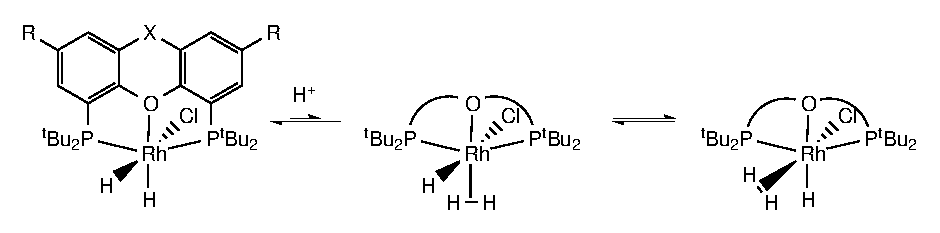
\includegraphics{../Schemes/Rhodiumdihydrogen.eps}
%\caption[Dynamic behaviour of rhodium dihydrogen complexes]{Dynamic behaviour of rhodium dihydrogen complexes.}
%\vspace{0.2cm}
%\label{rhodiumdihydrogen}
%\end{center}
%\end{scheme}
%\vspace{0.2cm}
%
%\fixme{Kathryn thinks I should use the full ligand in all of them.}
%
%When \ce{HBF4.OEt2} was used instead of \ce{CH2(SO2CF3)2}, a peak for the free \ce{BF4-} counterion was not observed in the fluorine NMR spectra (expected at -151 ppm\cite{Feller2007})  Instead, the \fluorine{} NMR spectra show a number of peaks between -142 and -156 ppm, some of which are of similar intensities indicating the possibility of coupling to a rhodium centre.  In this case the \proton{} NMR spectra are very similar to the reaction with \ce{CH2(SO2CF3)2} indicating that an equilibrium has likely been established.  In this case however, once the chloride has dissociated a \ce{BF4-} ligand may coordinate in its place resulting in the mixture of species observed in the \fluorine{} NMR spectra.   However, rhodium complexes with monodentate \ce{BF4-} ligands coordinated through one of the fluorine atoms generally appear between -164 and -160 ppm in the \fluorine{} NMR spectrum.\cite{Feller2007, Salem2006, Salem2008, Gandelman2003}
%
%%Negligible difference was observed in the \phosphorus{} NMR spectrum and the aromatic resonances of the \proton{} and \carbon{} NMR spectra (Table \ref{table:dihydrogen}).  However, the resonances for the \tBu{} and hydridic protons and carbons are very broad, coalescing to a single broad peak for the \tBu{} protons and two broad peaks for the \tBu{} carbons.  The hydridic protons appear in the same position as the dihydride however the well-resolved doublets-of-triplets-of-doublets have been replaced by two very broad singlets. 
%
%\begin{table}[htbp]
%\caption[Selected NMR data of rhodium dihydride and dihydrogen complexes]{Selected NMR data of rhodium dihydride and dihydrogen complexes} 
%\vspace{1em}
%\label{table:dihydrogen}
%\small
%\begin{center}
%\begin{tabular}{l c c c c}
%	\toprule{}
%	~~ & \multicolumn{2}{c}{\bfseries{Dihydride}} & \multicolumn{2}{c}{\bfseries{Protonated}}\\
%	\cmidrule(lr){2-3} \cmidrule(lr){4-5}
%	\bfseries{Diphosphine}&\bfseries{$\delta$\phosphorus{}$/$ppm}&\bfseries{\JRhP$/$Hz}&\bfseries{$\delta$\phosphorus{}$/$ppm}&\bfseries{\JRhP$/$Hz}\\
%	\midrule{}
%	\tBuSixantphos	&	78.2	&	116.1	&	78.1		&	115.6\\
%	\tBuThixantphos& 	77.8	&	117.8	&	77.7		&	115.7\\
%	\tBuXantphos	&	79.0	&	117.0	&	78.9		&	115.6\\
%	\bottomrule{}
%\end{tabular}
%\end{center}
%\end{table}

\section{Rhodium Carbonyl Complexes}

Metal carbonyl complexes are some of the most well-studied transition metal complexes for many reasons.  Metal carbonyls are involved in a number of different catalytic processes including hydroformylation, hydroesterification and hydrocarboxylation to introduce oxygen functionality.\cite{Leeuwenbook2000, Guiu2006, Bertoux1999}  These reactions are of great synthetic importance and numerous industrial examples are known, such as the conversion of a benzylic alcohol to a carboxylic acid using a palladium catalyst in the synthesis of ibuprofen\cite{Kjonaas2011} and the hydroformylation of 1,3-butadiene to adipaldehyde, an intermediate for producing caprolactam and \gls{HMDA}, key monomers for nylon-6.6 and nylon-6 manufacture.\cite{Franke2012}  These catalytic processes involve the terminal coordination of the carbonyl to the metal centre.  However, carbonyls can also act as bridging ligands, either solely through the carbon atom or in a side-on \hapto{2} mode involving the $\pi$-system.  

%hexamethylene-1,6-diamine (HMDA)

Transition metal carbonyl complexes have also been studied to investigate the electronic influence of other ligands.  The stretching frequency of the \ce{C#O} bond is a good measure of the electronic environment as carbonyl ligands are strong $\pi$-acceptor ligands, meaning that the metal centre will donate electron density into the $\pi^*$-orbital.  This weakens the \ce{C#O} bond and results in a shift of the infrared \ce{C#O} stretch to lower frequency.  The degree to which the back-bonding occurs is related to the nature of the metal centre and the other ligands.  As such, a number of series exist where this stretch has been used to quantify the electron donor capabilities of various ligands.  These include the well-known Tolman Electronic Parameter using \ce{[Ni(CO)3L]} complexes,\cite{Tolman1977, Tolman1970} and \ce{[Mo(CO)5L]} and \ce{[Rh(CO)ClL2]} series,\cite{Banger2009}  although other methods are utilised such as the phosphine selenide coupling constants (see Section \ref{section:selenides}) and the \JPtP{} coupling in \cis-\ce{[PtCl2P2]} complexes.\cite{Pregosin2012}

The typical method for producing rhodium phosphine carbonyl complexes is to react the free phosphine or diphosphine ligand with either the chloro-bridged dicarbonyl dimer, \ce{[Rh(CO)2Cl]2}, or by reaction with a chloro-bridged rhodium alkene dimer such as \ce{[Rh(C2H4)2Cl]2} or \ce{[Rh(coe)2Cl]2} under an atmosphere of carbon monoxide.  The reaction is then purified either in the air or under inert atmosphere and in the majority of cases the product is \trans-\ce{[Rh(CO)(PP)Cl]} where PP is either two monophosphine ligands or a \trans-spanning diphosphine.  Using smaller bite-angle diphosphine ligands results in the \cis{} isomer.  

The reactivity of the [Rh(\tBuxantphosk)Cl] complexes towards carbon monoxide was investigated on an NMR scale by bubbling CO through a \ce{C6D6} solution of the complex for 10 minutes before sealing the NMR tube with a J. Young tap.  An immediate colour change was observed, with the dark brown starting material changing to yellow (\tBusixantphos) or orange (\tButhixantphos{} and \tBuxantphos).  NMR analysis of these samples showed the reaction was complete, forming a single product in under 15 minutes with no evidence of the starting material.

The NMR spectra for the three resulting products show some differences.  The \proton{} and \carbon{} NMR spectra for the reaction of [Rh(\tButhixantphosk)Cl] with CO is broad, while the \phosphorus{} NMR spectrum shows only slight broadening.  This indicates possible dynamic behaviour.  However, the spectra for the reaction of [Rh(\tBusixantphosk)Cl] and [Rh(\tBuxantphosk)Cl] with CO are both well resolved (Figure \ref{Rhcarbonylnmr} shows a selection of the NMR spectra for the \tBuxantphos{} complex).  In all cases the \phosphorus{} NMR spectrum show a single peak at 69.3--71.6 ppm, split into a doublet by rhodium coupling of 120.0--122.2 Hz (Table \ref{table:rhodiumcarbonyl}).  These are shifted downfield relative to the [Rh(\tBuxantphosk)Cl] starting material.  The value of \JRhP{} has decreased from the starting [Rh(\tBuxantphosk)Cl] complexes from 140--142.3 Hz to 120.0--122.2 Hz.

\begin{figure}[htbp]
\begin{center}
\vspace{0.5cm}
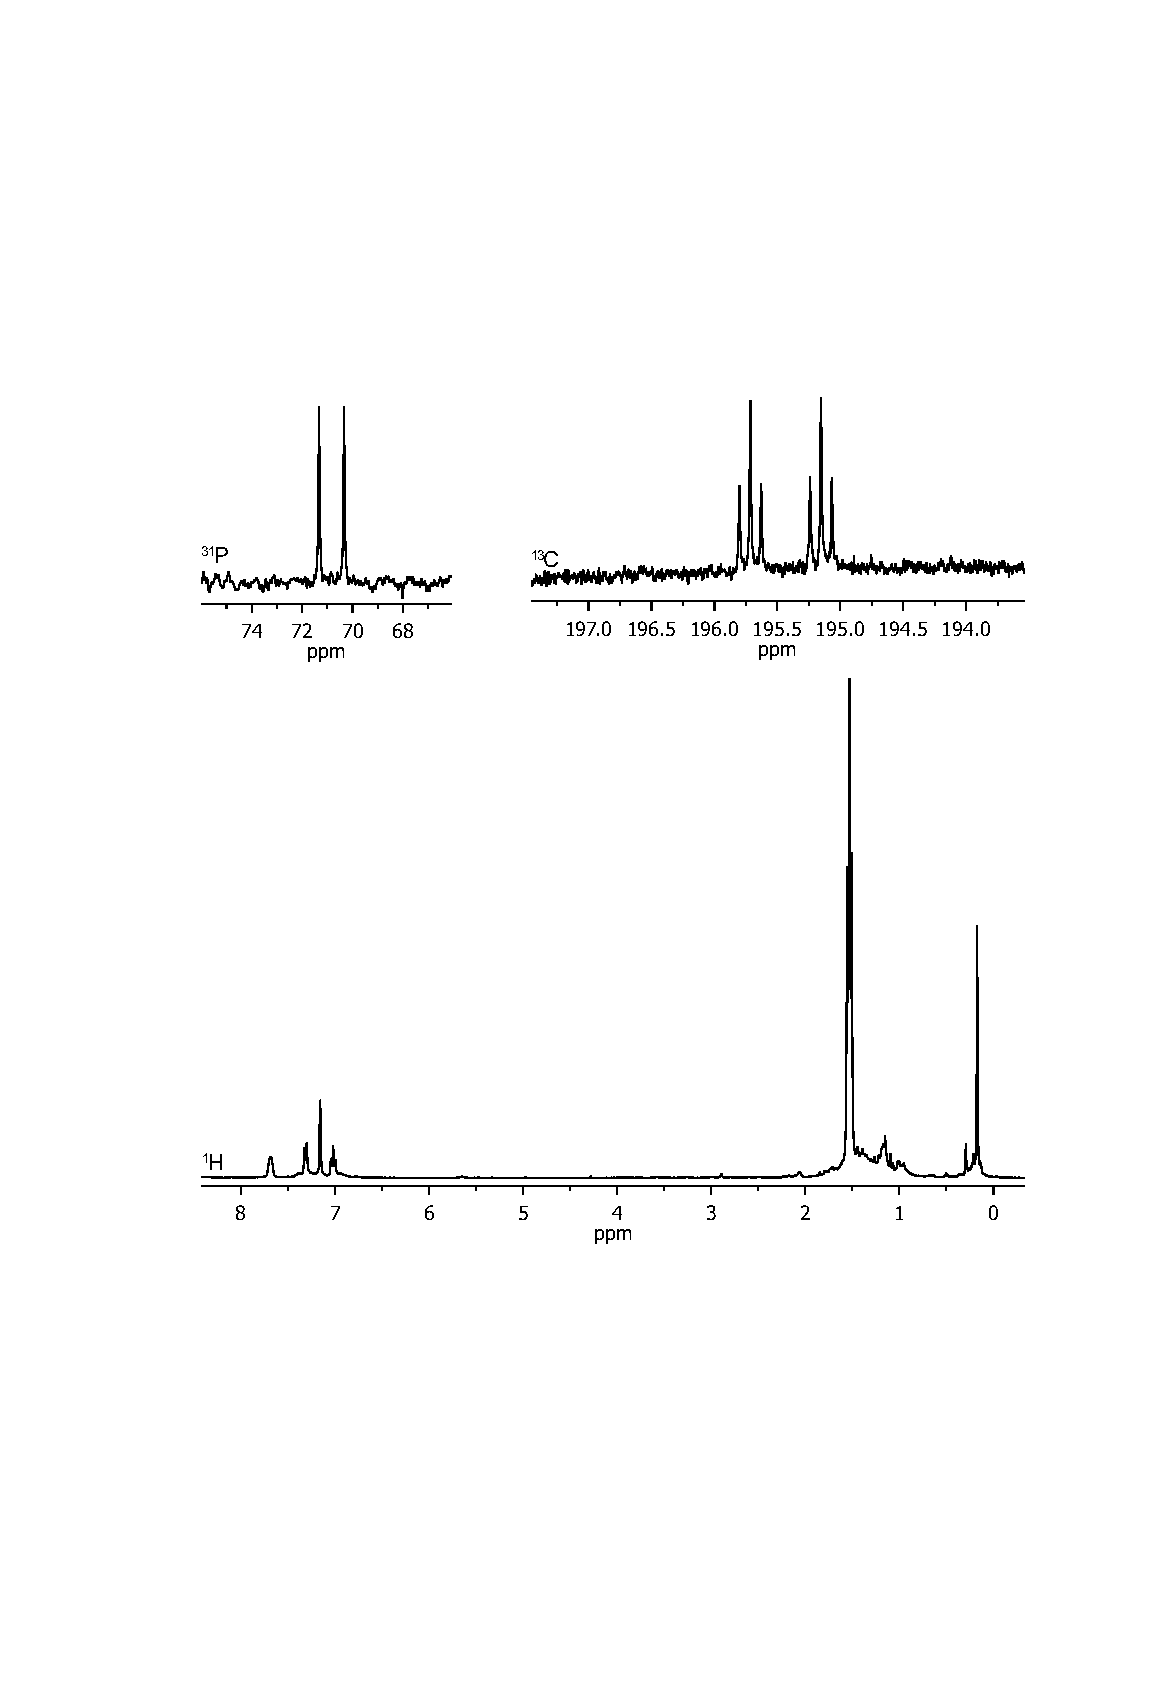
\includegraphics[trim = 2.5cm 7.2cm 2.5cm 5.0cm, clip]{../NMR/7017.eps}
\caption[NMR spectra of [Rh(\tBusixantphos)Cl{]} with CO]{\phosphorus, \carbon{} and \proton{} NMR spectra of the reaction of [Rh(\tBusixantphos)Cl] with CO in \ce{C6D6}.}
\vspace{0.2cm}
\label{Rhcarbonylnmr}
\end{center}
\end{figure}
\vspace{0.2cm}

%\fixme{Check that these spectra are all for the same compound}

\begin{table}[htbp]
\caption[Selected NMR data of [Rh(\tBuxantphos)\ce{(CO)2Cl}{]} complexes]{Selected NMR data of [Rh(\tBuxantphos)\ce{(CO)2Cl]} complexes in \ce{C6D6}.}
\vspace{1em}
\label{table:rhodiumcarbonyl}
\small
\begin{center}
\begin{tabular}{l c c c c c c}
	\toprule{}
	~ & \multicolumn{3}{c}{\bfseries{\phosphorus}} & \multicolumn{3}{c}{\bfseries{\carbon{} CO}} \\
	\cmidrule(lr){2-4} \cmidrule(lr){5-7}
	\bfseries{Ligand}&\bfseries{$\delta/$ppm}&\bfseries{$\Delta\delta$ ppm}&\bfseries{\JRhP{}$/$Hz}&\bfseries{$\delta/$ppm}&\bfseries{\JRhC $/$Hz}&\bfseries{\JPC $/$Hz}\\
	\midrule
	\tBuSixantphos	&	70.8	&	26.6 & 120.0	&	195.5	& 84.4	& 13.0\\
	\tBuThixantphos	& 	69.3	&	22.8	& 122.2	&	\multicolumn{3}{c}{not observed}\\
	\tBuXantphos	&	71.6	&	23.9	& 120.0	&	194.9	& 84.4	& 12.4\\
	\bottomrule{}
\end{tabular}
\end{center}
\end{table}

%\fixme{talk about the coupling constant relative to other rhodium carbonyl complexes}

The NMR spectra of the products from the reaction of the [Rh(\tBuxantphos)Cl] complexes with CO, indicate a high level of symmetry in the products.  In the \proton{} NMR spectra a single peak was observed for the \tBu{} groups and a singlet for the methyl groups for each of the three ligands.  The number of aromatic signals in the \proton{} NMR spectra indicate that two mirror planes exist, parallel to the backbone of the ligand and perpendicular to it (running through the oxygen and other bridging atom).  For \tBusixantphos{} and \tBuxantphos{} the \tBu{} groups appear as a virtual triplet indicating a \trans{} or pseudo \trans{} coordination geometry.  For \tButhixantphos{} the \tBu{} resonance displays some broadening, resulting in a singlet.

The number of signals in the \carbon{} NMR spectra is also suggestive of a highly symmetric product. Although the peaks were well resolved for the \tBusixantphos{} and \tBuxantphos{} complexes, in the \tButhixantphos{} complex all of the \carbon{} NMR peaks were broad except two, which can be attributed to the methyl groups and the aromatic carbon they are attached to, indicating that these carbons are unaffected by the dynamic process which leads to the broadening in this spectra.  This process may be either exchange of the CO ligand with the uncoordinated CO, or a change in geometry such as a trigonal bipyramidal to square-planar equilibrium.  

The reaction of the [Rh(\tBuxantphos)Cl] complexes with carbon monoxide was carried out with natural abundance CO.  Despite this, a peak was observed for the coordinated carbonyl in the \carbon{} NMR spectra for the \tBusixantphos{} and \tBuxantphos{} products (Table \ref{table:rhodiumcarbonyl} and Figure \ref{Rhcarbonylnmr}).  This peak occurs at 195.5 ppm for \tBusixantphos{} and 194.9 ppm for \tBuxantphos{} as a well resolved doublet of triplets indicating coupling to rhodium (\JRhC{} = 84.4 Hz for both) and two equivalent phosphorus atoms (\JPC{} = 13.0 and 12.4 Hz for \tBusixantphos{} and \tBuxantphos{} respectively).  These values are within the expected ranges for rhodium carbonyl complexes.  

%As coupling constants are heavily influenced by the ligand in the \trans{} position it is likely that the carbonyl is in the same environment in both complexes likely a \cis{} position relative to the phosphorus atoms as a \trans{} coordination to either the phosphorus or oxygen donor atoms would likely result in a change in the value of \JRhC{}.  However, in this particular case the \phosphorus{} NMR spectrum for the \tBusixantphos{} and \tBuxantphos{} complexes display identical \JRhP{} values.  

% \fixme{talk about the position of the carbonyl peak and the values of the coupling constants}

There are a number of different possible products for the reaction of the [Rh(\tBuxantphosk)Cl] complexes with carbon monoxide, due to the ability of rhodium(I) to form both square planar and trigonal bipyramidal structures, combined with the potential hemilability of the \tBuxantphos{} oxygen resulting in a \dento{}\emph{P,P}\textprime{} bonding geometry.  In addition, it is possible for either one or two carbonyl ligands to coordinate, displacing either the oxygen or the chloride ligand.  The number of possibilities is decreased by the inability for the \tBuxantphos{} ligands to coordinate in a \cis{} geometry on square planar centres (See Chapter \ref{ch:platinumII} for further discussion) thus also eliminating trigonal bipyramidal products with the \tBuxantphos{} complex coordinated in a \dento{}\emph{P,P}\textprime{} axial-equatorial position.  Possible products from the reaction are outlined in Figure \ref{RhCOpossibilities}.

\begin{figure}[htb]
\begin{center}
\vspace{0.5cm}
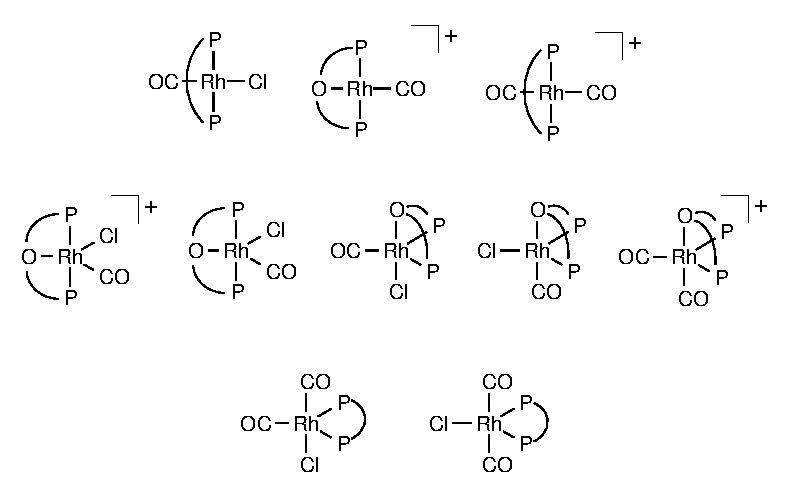
\includegraphics{../Figures/RhCOpossibilities.eps}
\caption[Possible products from reaction of \texorpdfstring{[Rh(\tBuxantphosk)Cl{]} complexes with CO} R]{Possible products from reaction of \texorpdfstring{[Rh(\tBuxantphosk)Cl] complexes with CO} R.  First row: square planar complexes, second row: trigonal bipyramidal complexes with \POP{} \tBuxantphos{}, and third row: trigonal bipyramidal complexes with \dento{}\emph{P,P}\textprime{} \tBuxantphos{} ligands.}
\vspace{0.2cm}
\label{RhCOpossibilities}
\end{center}
\end{figure}
\vspace{0.2cm}

The majority of the possible structures outlined in Figure \ref{RhCOpossibilities} can be discounted as they do no meet the symmetry requirements determined from the NMR spectra.  The only complexes consistent with the NMR spectra are the square planar complexes, [Rh(\tBuxantphosk)CO]Cl and [Rh(\tBuxantphos-\dento{}\emph{P,P}\textprime)\ce{(CO)2]Cl}; and the trigonal bipyramidal complexes, \trans-[Rh(\tBuxantphos-\dento{}\emph{P,P}\textprime)\ce{(CO)2Cl]} and [Rh(\tBuxantphosk)\ce{(CO)2]+}.  The mass spectra of the products from the reaction of the [Rh(\tBuxantphos)Cl] complexes with CO show a single major ion cluster.  This cluster only differs for the three ligands due to the differences in the ligand structure.  The cluster is consistent with a [Rh(\tBuxantphos)\ce{(CO)]+} ion in both mass/charge ratio and isotopic distribution.  While this supports the formulation of the product as a monocarbonyl entity, this ion cluster could result from any of the possible structures given in Figure \ref{RhCOpossibilities} as mass spectrometry is performed under high vacuum, which may result in loss of CO from the dicarbonyl structures, and ionisation by loss of chloride ligands is very common for coordination complexes.\cite{Henderson1998}

As previously discussed (Section \ref{section:rhodiumchloride}) the position of the \emph{O}-\emph{ipso} carbon peak in the \carbon{} NMR spectra for \tBuxantphos{} complexes can be used as a guide for the bonding mode of the ligand.  A peak for the  \emph{O}-\emph{ipso} carbon that has not shifted significantly from the \emph{O}-\emph{ipso} carbon peak for the free ligand is indicative of a \dento{}\emph{P,P}\textprime{} coordination, while a peak shifted downfield by more than 2.0 ppm is indicative of a \dento{}P,O,P\textprime{} coordination.   The products from this reaction show very little change in the position of the \emph{O}-\emph{ipso} peak compared to the free ligand (Table \ref{table:RhcarbonylOpeak}).  Thus indicating that the  coordination mode of the three \tBuxantphos{} ligands in these carbonyl complexes is most likely to be a bidentate \dento{}\emph{P,P}\textprime mode.

\begin{sidewaystable}[htbp]
\caption[Chemical shift and coupling for the \emph{O}-\emph{ipso} carbon in \tBuxantphos{}, [Rh(\tBuxantphos)Cl{]} and carbonyl complexes]{\carbon{} Chemical shift and coupling for the \emph{O}-\emph{ipso} carbon in \tBuxantphos{}, [Rh(\tBuxantphos)Cl{]} and carbonyl complexes.}
\vspace{1em}
\label{table:RhcarbonylOpeak}
\small
\begin{center}
\begin{tabular}{ c c c c c c c c c}
	\toprule{}
~&\multicolumn{2}{c}{\bfseries{Free ligand}} &\multicolumn{3}{c}{\bfseries{[Rh(\tBuxantphos)Cl]}}&\multicolumn{3}{c}{\bfseries{[Rh(\tBuxantphos)\ce{(CO)2Cl]}}}\\  
	\cmidrule(lr){2-3} \cmidrule(lr){4-6} \cmidrule(lr){7-9}
	\bfseries{Ligand}&\bfseries{$\delta$\carbon{}$/$ppm}&\bfseries{\J{}$/$Hz}&\bfseries{$\delta$\carbon{}$/$ppm}&\bfseries{$\Delta\delta$}&\bfseries{\J{}$/$Hz}&\bfseries{$\delta$\carbon{}$/$ppm}&\bfseries{$\Delta\delta$}&\bfseries{\J{}$/$Hz}\\
	\midrule{}
	\tBuSixantphos	&	164.3	& 11.3	&	169.5	& 5.2		& 14.4	& 164.3	& 0.0 	& 8.1 \\
	\tBuThixantphos	&	155.3	& 13.0	&	157.4	& 2.1 	& 16.8 	& 154.9	& -0.4 &n.o. \\
	\tBuXantphos	&	155.8	& 12.0	&	158.9	& 3.1		& 16.3	& 155.6	& -0.2	& 10.4 \\
	\bottomrule{}
\end{tabular}
\end{center}
\end{sidewaystable}
%\fixme{make some note about the delta delta values being from the free ligand}

The two possible square planar complexes [Rh(\tBuxantphosk)CO]Cl and [Rh(\tBuxantphos-\dento{}\emph{P,P}\textprime)\ce{(CO)2]Cl} and one of the trigonal bipyramidal structures [Rh(\tBuxantphosk)\ce{(CO)2]Cl} are positively charged.  As such, we would expect them not to be soluble in \ce{C6D6}.  However, the product of this reaction remains in a \ce{C6D6} solution with no signs of precipitation over a period of several weeks.  This supports the formulation of the product as the trigonal bipyramidal \trans-[Rh(\tBuxantphos)\ce{(CO)2}Cl].  Rhodium dicarbonyl complexes are typically only stable below room temperature and under an atmosphere of carbon monoxide, readily losing CO under vacuum.\cite{Sanger1984, Sanger1985}  No change was observed in the \phosphorus{} or \proton{} NMR spectra for the complexes in a \ce{C6D6} solution under an argon atmosphere after being under vacuum overnight.  Likewise no change was observed for these samples after several weeks in a \ce{C6D6} solution under argon.  

The \gls{IR} spectra of the [Rh(\tBuxantphos)\ce{(CO)2}Cl] complexes were obtained to determine any differences in the electronic properties of the three ligands.  The \ce{C#O} stretching frequency is sensitive to changes in the electron density on the metal centre.  More electron rich metal centres will enhance the back-donation from the metal into the $\pi^*$-orbital on the carbonyl.  As this is an anti-bonding orbital, increased electron density will result in decreased bond order observed as a lower \ce{C#O} stretching frequency in the \gls{IR} spectra.  The \gls{IR} spectra for the three [Rh(\tBuxantphos)\ce{(CO)2}Cl] complexes showed multiple stretches in the region where \ce{C#O} stretches are observed.  Indicative of multiple carbonyl ligands.  The major \ce{C#O} stretch occurs at 1979 \si{\per\centi\metre} for all of the complexes irrespective of the \tBuxantphos{} ligand present.  This indicates that the ligands are comparable in their electron donation capabilities in the \dento{}\emph{P,P}\textprime{} coordination mode.  The presence of multiple carbonyl stretches in the \gls{IR} is further evidence for a dicarbonyl complex.  

Previous reports described the formation of \trans-{[Rh(CO)Cl(diphosphine)]} complexes upon reaction of \Phxantphos{} and DPEphos with \ce{[Rh(CO)2Cl]2}.\cite{Deb2010}  These complexes appeared in the \phosphorus{} NMR spectra at 27.3 and 22.6 ppm with \JRhP{} = 119.2 and 123.5 Hz for \Phxantphos{} and DPEphos respectively.  In the \carbon{} NMR spectra singlets were observed for the carbonyl ligands at 180.9 and 183.3 ppm for \Phxantphos{} and DPEphos respectively.  The position of the carbonyl carbon in the \tBuxantphos{} complexes is at 195.5 or 194.9 ppm, indicating less shielding, which may be a result of the more electron rich rhodium centre in a five-coordinate complex.  The rhodium chemistry of a more sterically demanding version of \Phxantphos{} where the phenyl rings are replaced with \emph{o}-tolyl groups has also been reported.\cite{Williams2011}  Again, this complex forms a \trans-[Rh(CO)Cl(diphosphine)] complex.  However, the analogous complexes with an iodide replacing the chloride ligand forms a square pyramidal structure with the oxygen coordinated to the rhodium.  The \ce{C#O} stretching frequencies for the \tBuxantphos{} carbonyl complexes (1979 \si{\per\centi\metre}) occur between those for the \trans-[Rh(CO)Cl(\Phxantphos)] (1974 \si{\per\centi\metre}) and \trans-[Rh(CO)Cl(DPEphos)] (1985 \si{\per\cm}).  The \ce{C#O} stretch is similar to [Rh(CO)Cl\ce{(PR3)2}] with \ce{PR3} = \ce{PPh3} (1979 \si{\per\centi\metre}) however, the strongly electron donating \tBu{} substituents on the \tBuxantphos{} ligands should result in a lower stretching frequency such as that where \ce{PR3} = \ce{PPhMe2} (1968 \si{\per\cm}).\cite{Banger2009}  This is further evidence that the \tBuxantphos{} complexes are not \trans-[Rh(\tBuxantphos)(CO)Cl].  

%%%%%%%\fixme{Kathryn may disagree with this logic}

Based on this evidence we propose that the reaction of the [Rh(\tBuxantphos)Cl] complexes results in a trigonal bipyramidal structure with the \tBuxantphos{} ligand occupying two of the equatorial sites in a \dento{}\emph{P,P}\textprime{} coordination mode.  The remaining equatorial site is occupied by a chloride ligand and carbonyl ligands take up the two axial positions (Scheme \ref{RhodiumCOscheme}).  Trigonal bipyramidal structures (particularly those with carbonyl ligands) are known to undergo facile rearrangement to square pyramids.\cite{Sanger1985} This may be the cause of the broadening of the spectra for the \tButhixantphos{} system, and the multiple peaks observed in the \gls{IR} spectra.  \Phxantphos{} and DPEphos both form \trans{}-[Rh(CO)Cl(diphosphine)], which would have a larger P-Rh-P angle than the [Rh(\tBuxantphos)(\ce{CO)2}Cl] complexes.  This is counterintuitive as the natural bite-angle is larger for the \tBuxantphos{} ligands than for \Phxantphos{}.  However, it is possible that the \trans{}-[Rh(CO)Cl(diphosphine)] are actually square pyramidal complexes with a weak interaction of the ether bridge in the diphosphine ligands, thus relieving the strain of such a wide bite-angle.

%Read Koga1988 about Berry pseudorotation

\begin{scheme}[htb]
\begin{center}
\vspace{0.5cm}
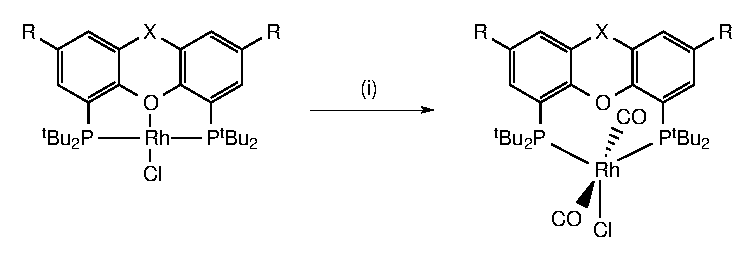
\includegraphics{../Schemes/Rhodiumcarbonyl.eps}
\caption[Reaction of \texorpdfstring{[Rh(\tBuxantphos)Cl{]}} R with carbon monoxide]{Reaction of \texorpdfstring{[Rh(\tBuxantphos)Cl{]}} R with carbon monoxide.  \emph{Reagents and conditions:} (i) 10 mins CO, \ce{C6D6}, 3 days.}
\vspace{0.2cm}
\label{RhCOscheme}
\end{center}
\end{scheme}
\vspace{0.2cm}

Dicarbonyl complexes have been reported for \Phxantphos{} ligands, for example, \Phsixantphos{}, \Phthixantphos{} and \Phxantphos{} form [Rh\ce{(CO)2}H(\Phxantphos)] complexes.\cite{Kranenburg1995}  The diphosphine ligands coordinate in a \emph{bis}-equatorial-\dento{}\emph{P,P}\textprime{} mode, while the hydride occupies an axial site and the two carbonyls are in one equatorial and one axial site.  Little difference is observed between the three ligands with the \phosphorus{} NMR peaks between 21.1 and 23.4 ppm (\JRhP = 123.9--127.9 Hz).  Interestingly, although the two carbonyl ligands are inequivalent, only one carbonyl peak was reported, occurring as a doublet of triplets at 201.1 ppm with \JRhC{} = 65.7 Hz, and \JPC = 10.6 Hz for the \Phxantphos{} complex.  No explanation was given for this but it may be due to the rapid exchange of one of the carbonyl ligands with free CO leading to broadening of the second \carbon{} peak.  

%%%%%%%%%\fixme{Kathryn think I need to justify why I don't have elemental analysis}

%\fixme{Still to come: Carbonyl IR results and theoretical analysis of the different structures}

\section{Dioxygen and Oxo Complexes}

The reaction of rhodium(I) complexes with oxygen is well established with numerous examples published.\cite{Valentine1973, Choy1972}  Many aspects of the oxidation of Wilkinson's complex (\ce{[RhCl(PPh3)3]}) to form a distorted octahedral complex with a side-on \hapto{2}-\ce{O2} ligand have been reported, including the synthesis\cite{Baird1966, Atlay1980}, degradation\cite{Atlay1983} and use as an oxidation catalyst.\cite{Carlton1983, Read1985}  Numerous other rhodium dioxygen complexes have been reported with monophosphine \cite{Ahijado2005, Aresta1987, Bennett1977, Busetto1977, Gaal1977, Richter2000, Selke1993, Selke1995, Teets2012, Wakatsuki1990} and diphosphine\cite{Banwell2003, James1980,  Mague1977, McGinnety1969, Miller1975, Morvillo1986, Pettinari2002, Slack1979} ligands.  Reports of rhodium dioxygen complexes with heterobidentate\cite{Kashiwabara1997, Lindner1993, Perera1995, Yu2006} and tridentate\cite{Doux2003, Frech2006, Hayashi2013, Lanci2006, Vasapollo1981, Verat2008, Vigalok1996} ligands are also numerous.  However, despite the number of rhodium complexes of \Phxantphos{} and other xantphos derivatives, no rhodium dioxygen complexes of these ligands have been reported.  To address this, the reactivity of 
the [Rh(\tBuxantphos)Cl] and [Rh(\tBuxantphos)Cl\ce{(H)2}] complexes with all three ligands towards oxygen was investigated.  

Bubbling air through a \ce{C6D6} solution of each of the [Rh(\tBuxantphosk)Cl] complexes resulted in the rapid formation of a new complex as expected (Scheme \ref{Rhodiumdioxygen}).  The dihydride complexes, [Rh(\tBuxantphosk)Cl\ce{(H)2}], also reacted rapidly with air to form the same complexes.  The \phosphorus{} NMR spectra of the resulting [Rh(\tBuxantphos)Cl(\hapto{2}-\ce{O2})] complexes showed a single doublet (39.4--40.5) shifted upfield from the [Rh(\tBuxantphos)Cl] complex by between 4.8 and 7.5 ppm (Table \ref{table:dioxygennmr}).  The value of \JRhP{} decreased by 37.8--41.6 Hz, to 100.7--102.2 Hz.  This is consistent with a change in the oxidation state from rhodium(I) to rhodium(III) and the corresponding decrease in the s-character of the metal hybrid orbital, resulting from the change in coordination geometry from square planar to pseudo-octahedral.  

\begin{scheme}[htb]
\begin{center}
\vspace{0.5cm}
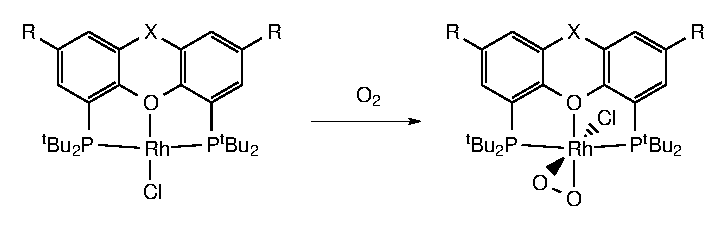
\includegraphics{../Schemes/Rhodiumdioxygen.eps}
\caption[Reaction of \texorpdfstring{[Rh(\tBuxantphos)Cl{]}} R complexes with oxygen]{Reaction of \texorpdfstring{[Rh(\tBuxantphos)Cl{]}} R complexes with oxygen. \emph{Reagents and conditions:} (i) 10 mins Air, \ce{C6D6}, 24 hours.}
\vspace{0.2cm}
\label{Rhodiumdioxygen}
\end{center}
\end{scheme}
\vspace{0.2cm}

%%%%%%%%%\fixme{Kathryn says needs a clearer line between the oxygens}

\begin{sidewaystable}[htbp]
\caption[Selected NMR data for [Rh(\tBuxantphosk)Cl($\eta^2$-\ce{O2}){]}]{Selected NMR data for [Rh(\tBuxantphosk)Cl($\eta^2$-\ce{O2})] in \ce{C6D6}.}
\vspace{1em}
\label{table:dioxygennmr}
\small
\begin{center}
\begin{tabular}{l c c c c c c c}
\toprule{}
	~~ & \multicolumn{4}{c}{\bfseries{\phosphorus}} & \multicolumn{3}{c}{\bfseries{\carbon{} \emph{O}-\emph{ipso}}}\\
	\cmidrule(lr){2-5} \cmidrule(lr){6-8}
	\bfseries{Diphosphine}&\bfseries{$\delta/$ppm}&\bfseries{$\Delta\delta/$ppm}&\bfseries{\JRhP$/$Hz}&\bfseries{$\Delta$ \JRhP$/$Hz}&\bfseries{$\delta/$ppm}&\bfseries{$\Delta\delta/$ppm}&\bfseries{\J{}$/$Hz} \\
	\midrule
	\tBuSixantphos 		& 39.4 & 4.8 & 102.2 & 37.8 & 166.7 & 2.4 & 9.8\\
	\tBuThixantphos 	& 39.0 & 7.5 & 101.5 & 40.0 & 155.9 & 0.6 & 12.5\\
	\tBuXantphos		& 40.5 & 7.2 & 100.7 & 41.6 & 157.3 & 1.5 & 11.5\\
	\bottomrule{}
\end{tabular}
\end{center} 
\end{sidewaystable}

The \proton{} and \carbon{} NMR spectra for the three [Rh(\tBuxantphos)Cl(\hapto{2}-\ce{O2})] complexes showed a loss of symmetry compared to the starting [Rh(\tBuxantphos)Cl] complexes.  A single peak was observed for the methyl substituents on the aromatic rings of the \tButhixantphos{}.  However, two peaks were present for the methyl substituents on the carbon or silicon bridging atoms in both the \tBuxantphos{} and \tBusixantphos{} complexes.  In all three complexes, two different sets of peaks for the \tBu{} groups were observed.  Together, this data indicates the presence of a plane of symmetry perpendicular to the backbone through the bridging atoms, and the absence of a plane of symmetry parallel to the backbone.  Interestingly, the two methyl groups in the \tBusixantphos{} and \tBuxantphos{} complexes occur in very different positions; one of the methyl groups is shifted upfield and the other downfield in both the \proton{} and \carbon{} NMR spectra, compared to the [Rh(\tBuxantphosk)Cl] starting material and [Rh(\tBuxantphosk)\ce{Cl(H)2]}.  The effect is more pronounced for \tBuxantphos{} than \tBusixantphos{}.  In addition, one of the \tBu{} groups in each of the three \tBuxantphos{} ligands is well resolved as a virtual triplet for all the \proton{} and \carbon{} NMR environments, while the other \tBu{} group has a well resolved virtual triplet for the quaternary carbon while the terminal carbon and protons are broad.
%
%\begin{table}[htbp]
%\caption[Comparison of the NMR data for the methyls in \tBusixantphos{} and \tBuxantphos{} rhodium complexes]{Comparison of the NMR data for the methyls in \tBusixantphos{} and \tBuxantphos{} rhodium complexes}
%\vspace{1em}
%\label{table:dioxygennmrmethyls}
%\small
%\begin{center}
%\begin{tabular}{ l c c c c}
%\toprule{}
%	~~ & \multicolumn{2}{c}{\bfseries{\proton}} & \multicolumn{2}{c}{\bfseries{\carbon}}\\
%		\cmidrule(lr){2-3} \cmidrule(lr){4-5}
%	\bfseries{Complex}&\bfseries{$\delta/$ppm}&\bfseries{$\delta/$ppm}&\bfseries{$\delta/$ppm}&\bfseries{$\delta/$ppm}\\
%		\midrule{}
%		{[}Rh(\tBuSixantphosk)Cl]			& 0.07&~ & -0.7~ &~ \\
%		{[}Rh(\tBuSixantphosk)Cl(H)\sub{2}]	& 0.17 & 0.10 & -0.7 & -0.9 \\
%		{[}Rh(\tBuSixantphosk)\ce{(CO)2}Cl]	& 0.18 & ~&-1.5 & ~\\
%		{[}Rh(\tBuSixantphosk)\hapto{2}-\ce{(O2)}Cl] & 0.19 & 0.01 & 0.8 & -4.2 \\
%		{[}Rh(\tBuXantphosk)Cl]			& 1.16 & ~ & 33.8 &~\\
%		{[}Rh(\tBuXantphosk)\ce{Cl(H)2}]		& 1.25 & 1.22 & 32.4 & 30.4 \\
%		{[}Rh(\tBuXantphosk)\ce{(CO)2}Cl]	& 1.24 & ~ & 31.4 &~ \\
%		{[}Rh(\tBuXantphosk)\hapto{2}-\ce{(O2)}Cl] & 1.43 & 1.00 & 35.5 & 24.2 \\
%	\bottomrule{}
%\end{tabular}
%\end{center} 
%\end{table}

%Unlike the complexes with iPr-xantphos the complexes \ce{[Rh($\eta^3-$tBu-xantphos)Cl]} were unstable in solution over prolonged periods.  Overnight a new resonance appeared in the \phosphorus NMR spectrum, shifted upfield with a much smaller coupling constant (\JRhP{} = 101.5 Hz).  This decrease in coupling constant is consistent with an increase in the oxidation state to rhodium(III).  However, this occurred in dry, degassed \ce{C6D6} which should not be reactive towards the complex.  No signals other than those expected for the ligand were observed in the \proton, \carbon, or \phosphorus{} NMR spectra.  

In the \carbon{} NMR spectra for the [Rh(\tBuxantphos)Cl(\hapto{2}-\ce{O2)}] complexes, the shift in the position of the \emph{O}-\emph{ipso} carbon peak from the free ligand was lower than for the [Rh(\tBuxantphos)Cl] complexes (Table \ref{table:dioxygennmr}).  In particular, the \tButhixantphos{} dioxygen complex exhibited a shift in position of only 0.6 ppm.  However, the effect is typically reduced for the \tButhixantphos{} ligand system, in fact for [Rh(\tButhixantphos)Cl\ce{(H)2}] a shift of only 0.1 ppm was observed despite a \POP{} coordination geometry.  This difference may be due to the electron donation from the methyl groups on the aromatic system of \tButhixantphos{}, which may mitigate the loss of electron density in the O-\emph{ipso} carbon upon oxygen coordination.  The shifts for \tBusixantphos{} and \tBuxantphos{} are both consistent with \POP{} coordination in the [Rh(\tBuxantphos)Cl(\hapto{2}-\ce{O2)}] complexes.  

Slow evaporation of a \ce{C6D6} solution of [Rh(\tBuxantphosk)Cl(\hapto{2}-\ce{O2})] produced dark red crystals suitable for X-ray diffraction.  The crystal structure (Figure \ref{Crystal:rhodium}) displayed some substitutional disorder with the dioxygen ligand replaced in approximately 15\% of the sites by an oxo ligand (Figure \ref{Crystal:rhodiumoxo}).  The complexes co-crystallised in the orthorhombic space group \emph{Pbca}.  Crystallographic data is given in Table \ref{crystal:rhodium:data} and selected bond lengths and angles are given in Table \ref{crystal:rhodium:lengths}.

%rhodium(III) complex.  The crystal structure (Figures \ref{Crystal:rhodium}) revealed the presence of a coordinated dioxygen molecule.  The complex crystallised as \ce{[Rh(tBu-xantphos)Cl(}$\eta_2$\ce{-O2})] in the orthorhombic space group \emph{Pbca}.  Selected bond lengths and angles are given in Table \ref{crystal:rhodium:lengths} and crystallographic data is given in Table \ref{crystal:rhodium:data}.  This complex likely formed by slow diffusion of oxygen through the septum sealing the NMR tube.  The crystal structure showed some substitutional disorder with the peroxo ligand substituted for an oxo ligand in approximately 15\% of the sites.  Selected bond lengths and angles for the oxo complex are given in Table \ref{crystal:rhodium:lengths:oxo}.

\begin{figure}[htbp]
\begin{center}
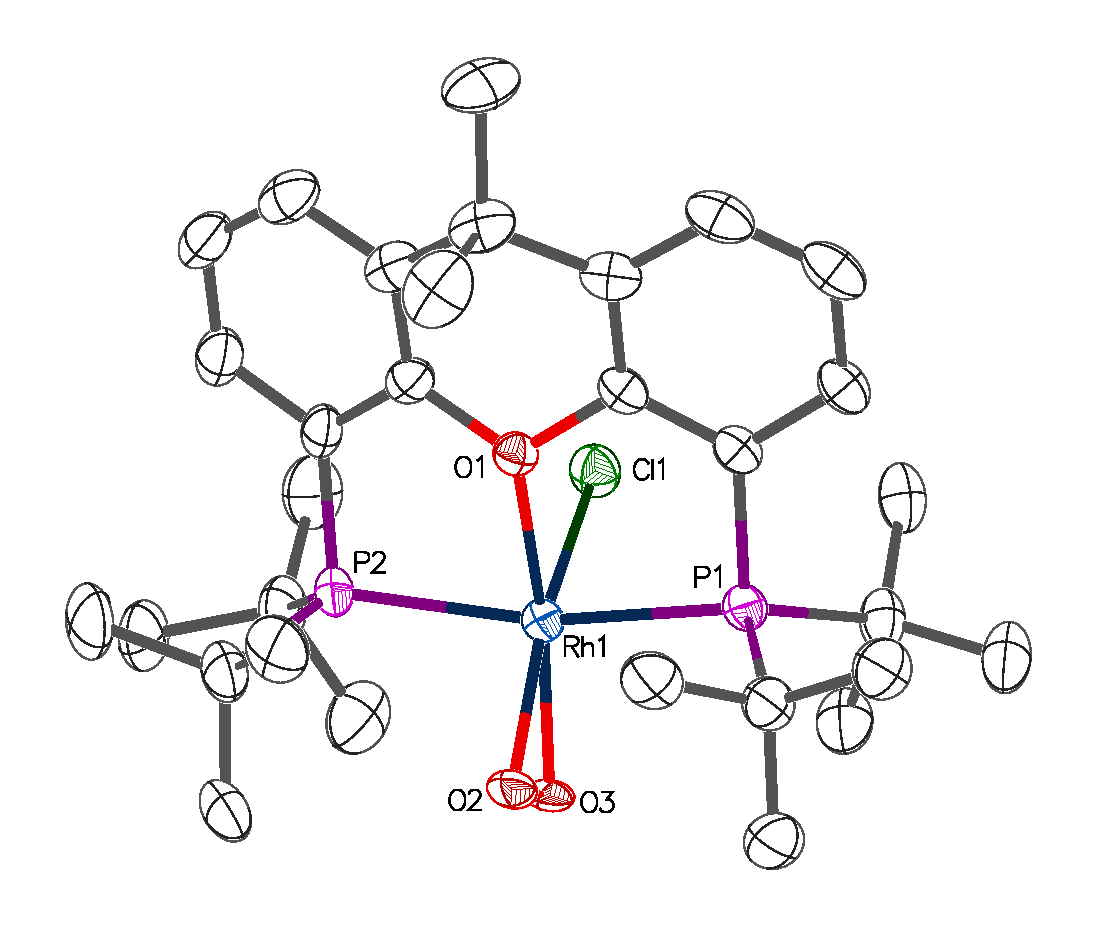
\includegraphics[scale=0.55]{../Crystalstructures/MRMN-Ga-dioxygen.eps}
\caption[X-ray crystal structure of [Rh(\tBuxantphos)Cl($\eta^2$-\ce{O2}){]}]{X-ray crystal structure of [Rh(\tBuxantphos)Cl($\eta^2$-\ce{O2})], hydrogen atoms omitted for clarity.}
\label{Crystal:rhodium}
\end{center}
\end{figure}

\begin{figure}[hbtp]
\begin{center}
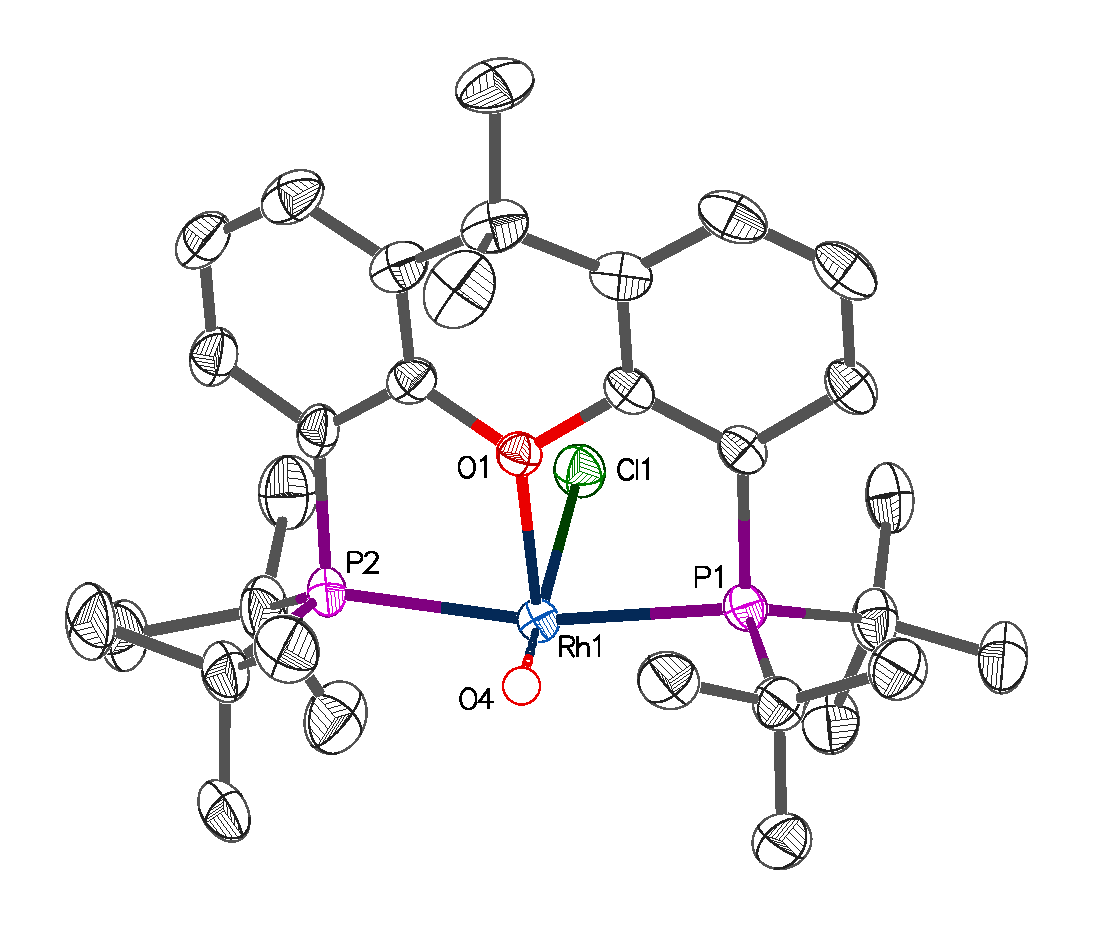
\includegraphics[scale=0.55]{../Crystalstructures/MRMN-Ga-oxo.eps}
\caption[X-ray crystal structure of [Rh(\tBuxantphosk)Cl(O)]{X-ray crystal structure of [Rh(\tBuxantphosk)Cl(O)], hydrogen atoms omitted for clarity.}
\label{Crystal:rhodiumoxo}
\end{center}
\end{figure}

%\begin{figure}[htp]
%\begin{center}
%\vspace{0.5cm}
%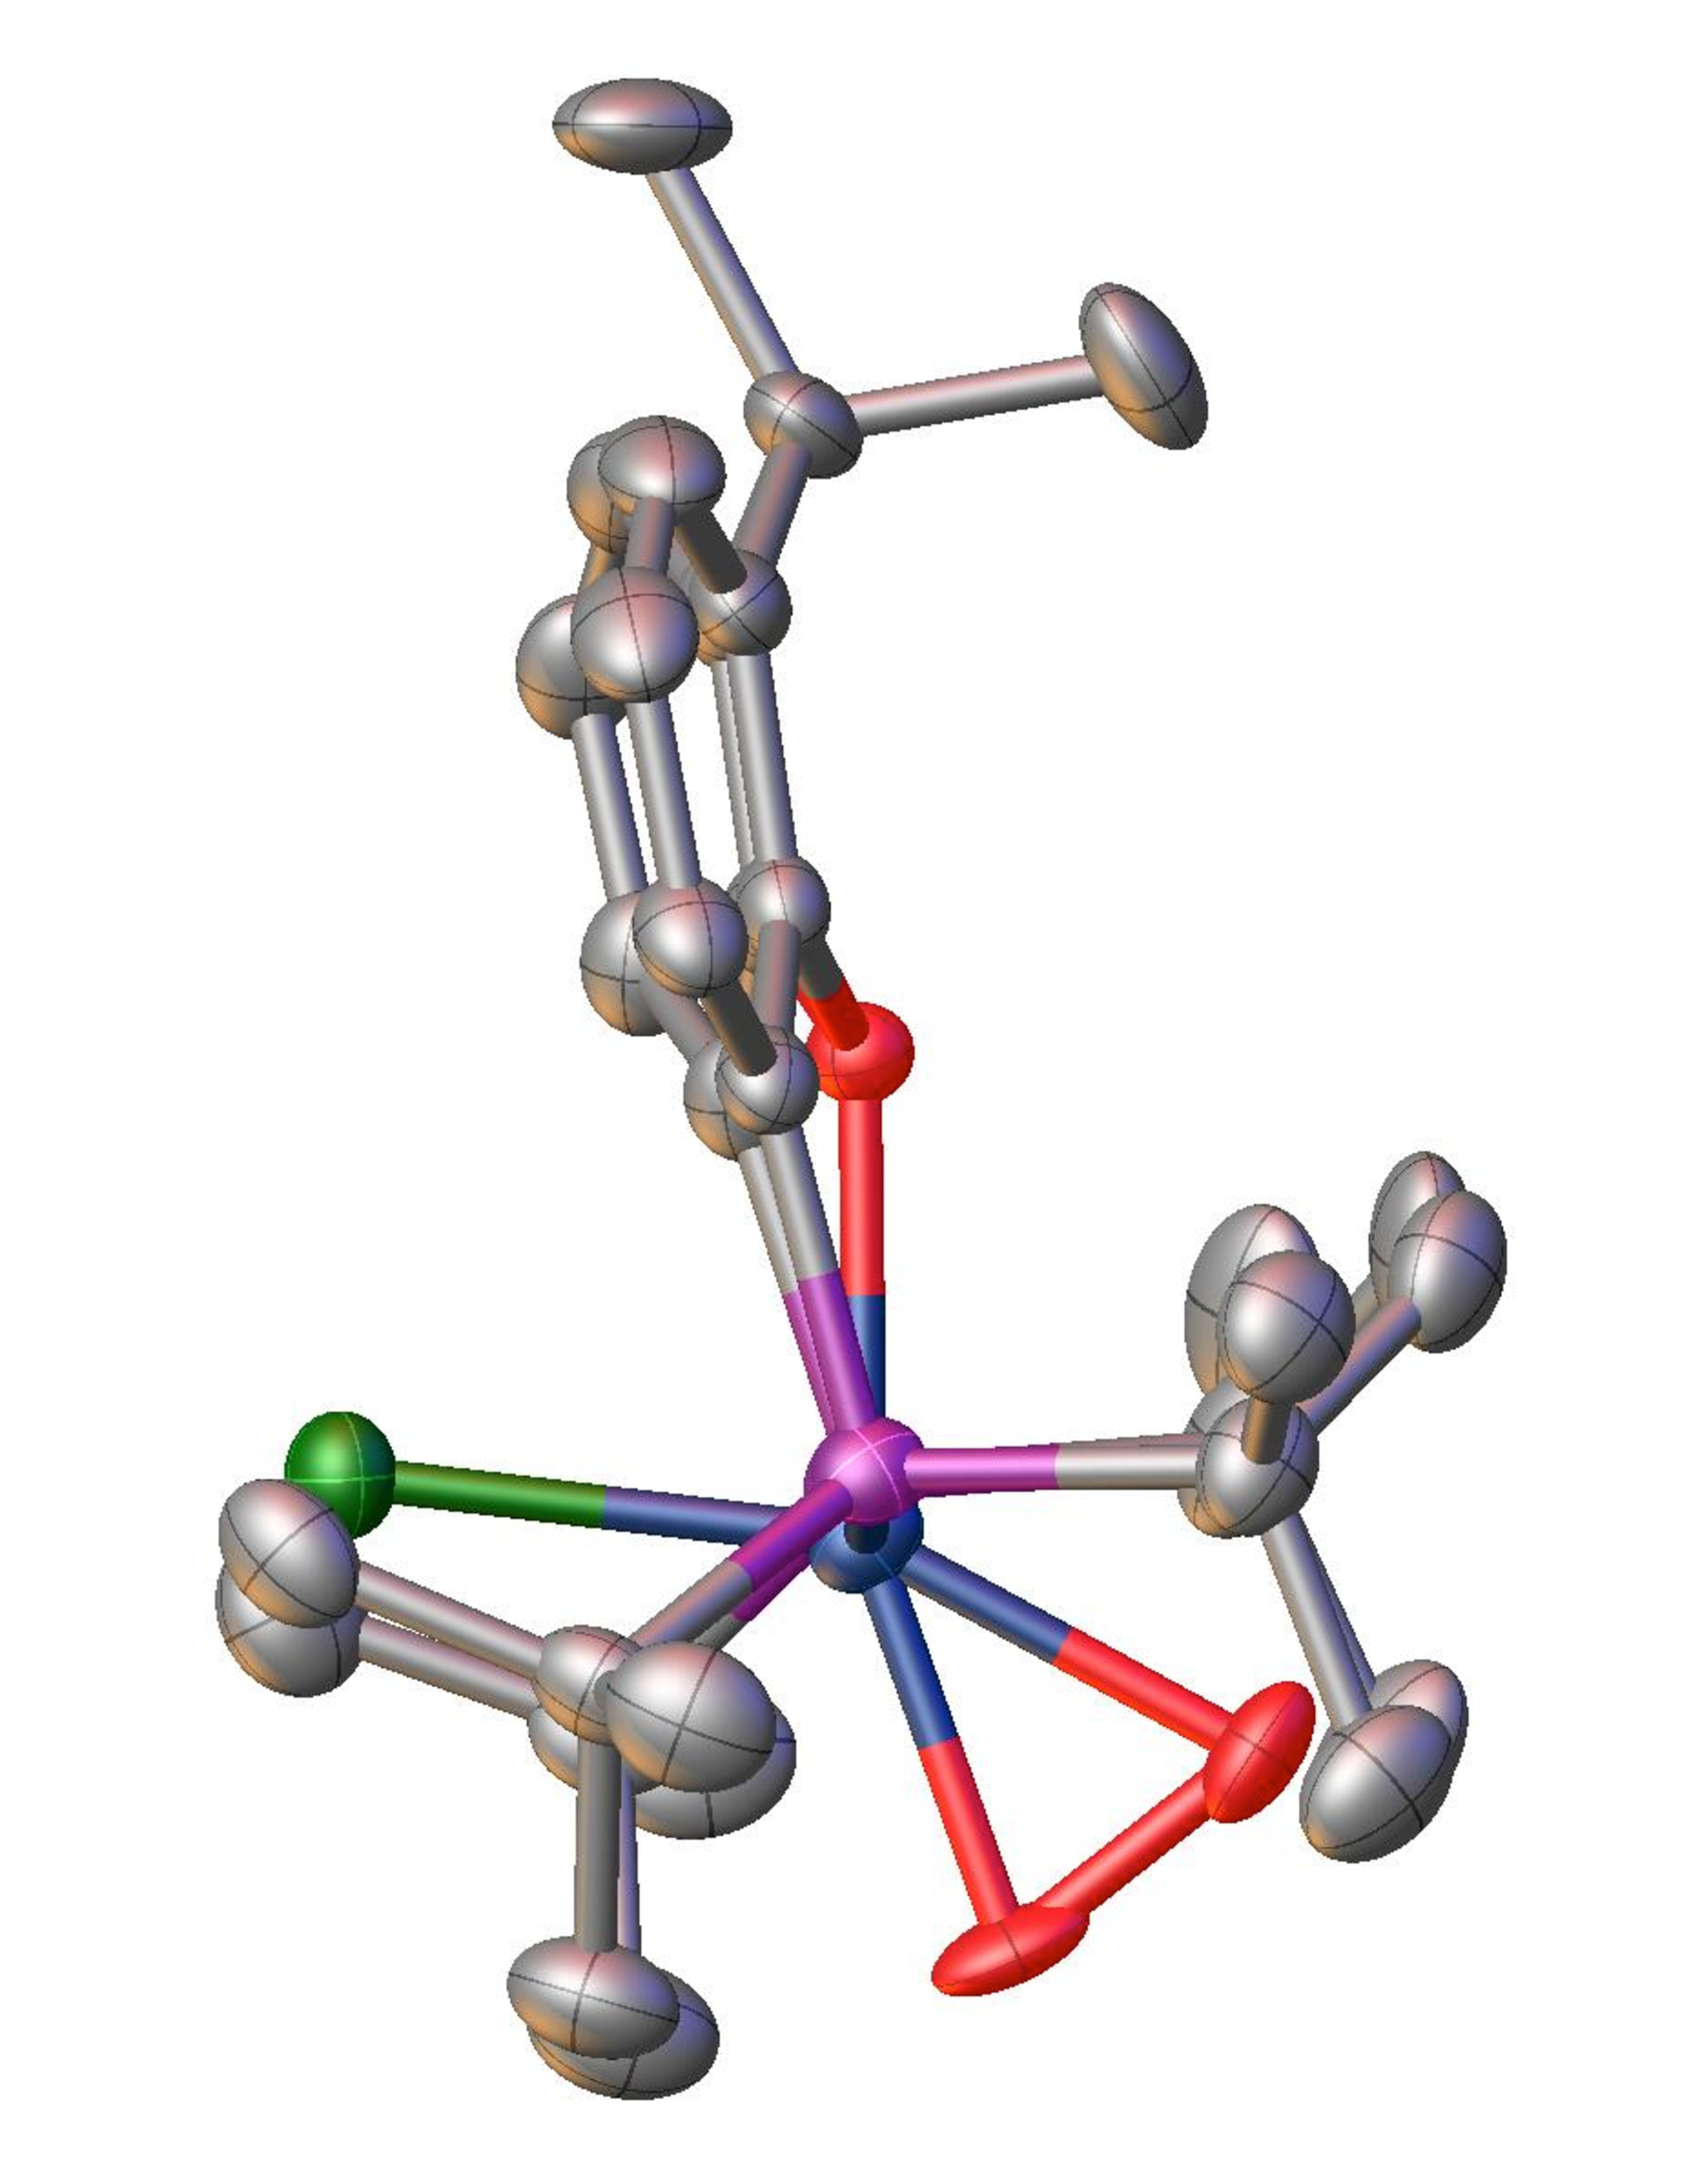
\includegraphics[width=0.4\textwidth]{../Figures/Crystalrhodiumside.pdf}
%\caption[X-ray crystal structure of \ce{[Rh(tBu-xantphos)Cl(}$\eta^2$\ce{-O2}){]} - side view]{X-ray crystal structure of \ce{[Rh(tBu-xantphos)Cl(}$\eta^2$\ce{-O2})], hydrogen atoms omitted for clarity - side view}
%\vspace{0.2cm}
%\label{Crystal:rhodiumside}
%\end{center}
%\end{figure}
%\vspace{0.2cm}

\begin{table}[htbp]
\small
\caption[Crystallographic data and structure refinement of [Rh(\tBuxantphos)Cl(\hapto{2}-\ce{O2}){]}]
{Crystallographic Data and Structure Refinement of [Rh(\tBuxantphos)Cl(\hapto{2}-\ce{O2})].}
\vspace{1em}
\label{crystal:rhodium:data}
\small
\begin{center}
\begin{tabular}{l l}
	\toprule
	\bfseries{Empirical formula}~~& \bfseries{\ce{C31H48ClO_{2.85}P2Rh}}\\
	\midrule
	Formula weight	 							& 666.53\\
	Temperature/K	 							& 120.01(10)\\
	Crystal system	 							& orthorhombic\\
	Space group	 							& Pbca\\
	a$/$\si{\angstrom}							& 11.84223(17)\\
	b$/$\si{\angstrom} 							& 20.2961(3)\\
	c$/$\si{\angstrom}							& 26.8069(4)\\
	$\alpha/$\degrees							& 90\\
	$\beta/$\degrees							& 90\\
	$\gamma/$\degrees							& 90\\
	Volume$/$\si{\angstrom\cubed}  				& 6443.06(17)\\
	Z	 									& 8\\
$\rho$\sub{calc} \si{\milli\gram}$/$\si{\milli\metre\cubed} 	& 1.374\\
\si{\metre}$/$\si{\milli\metre} 						& 6.206\\
F(000)	 									& 2790.0\\
Crystal size$/$\si{\milli\metre\cubed}	 				& 0.1092 x 0.0738 x 0.0159\\
Radiation	 									& CuK$\alpha$ ($\lambda$ = 1.54184)\\
2$\theta$ range for data collection					& 6.594 to 147.8\degrees\\
Index ranges	 								& -14 $\leq$ h $\leq$ 13, -25 $\leq$ k $\leq$ 21, -30 $\leq$ l $\leq$ 33\\
Reflections collected	 							& 45616\\
Independent reflections	 						& 6481 [R\sub{int} = 0.0631, R\sub{sigma} = 0.0332]\\
Data$/$restraints$/$parameters					& 6481$/$399$/$367\\
Goodness-of-fit on F$^{2}$	 					& 1.035\\
Final R indexes [I$>$=2$\sigma$ (I)]	 				& R\sub{1} = 0.0439, wR\sub{2} = 0.1145\\
Final R indexes [all data]	 						& R\sub{1} = 0.0550, wR\sub{2} = 0.1226\\
Largest diff. peak/hole / e \si{\per\angstrom\cubed}		& 1.40/-0.78	\\
	\bottomrule
\end{tabular}
\end{center}
\end{table}

\begin{table}[htp]
\caption[Selected bond distances (\AA) and angles (\degrees) of [Rh(tBu-xantphos)Cl($\eta^2$-\ce{O2}){]}]{Selected bond distances (\AA) and angles (\degrees) of [Rh(\tBuxantphos)Cl($\eta^2$-\ce{O2})].}
\vspace{1em}
\label{crystal:rhodium:lengths}
\small
\begin{center}
\begin{tabular}{l l l l}
	\toprule
	\multicolumn{2}{l}{\bfseries{~Bond distances (\si{\angstrom})}} & \multicolumn{2}{c}{\bfseries{Bond angles (\degrees)}} \\
	\midrule		
	P1-Rh & 2.3391(8)	& P1-Rh-P2 & 166.01(3) \\
	P2-Rh & 2.3237(9)	& Cl1-Rh-O2 & 158.18(10)\\
	O1-Rh & 2.193(2)	& Cl1-Rh-O4 & 161.2(3)\\
	O2-Rh & 2.016(3)	& O1-Rh-O3 & 161.33(12)\\
	O3-Rh & 1.962(3)	& Ring1-Ring2 & 26.65(12)\\
	Cl1-Rh & 2.3871(9)	& O1-C(bridge)-\ce{CH3} & 165.9(3)\\
	O2-O3 & 1.424(5)	& O1-C(bridge)-\ce{CH3} & 94.7{3}\\
	O4-Rh & 1.669(10)	& & \\
	\bottomrule{}
\end{tabular}
\end{center}
\end{table}

The O-O bond lengthens upon coordination due to back-bonding from the metal into the anti-bonding $\pi^*$-orbital of the ligand.  In the crystal structure of [Rh(\tBuxantphos)Cl($\eta^2$-\ce{O2})], the O2-O3 bond length is 1.424(5) \si{\angstrom}, lengthened by 0.21 \si{\angstrom} from the bond length in molecular oxygen of 1.21 \si{\angstrom}.\cite{SI2002}  This length is typical for rhodium dioxygen complexes with the average O-O bond length being 1.423 \A.\cite{Allen2002}  The Rh-O bond lengths for the dioxygen ligand are different, with the oxygen \trans{} to chloride having a longer bond by 0.054 \A.  The oxygen \trans{} to chloride has a typical Rh-O bond length for rhodium dioxygen complexes (average = 2.017 \A), while the oxygen \trans{} to the ether bridge is shorter than average with a length of 1.962(3) \A.  This shorter bond results from the low \trans-influence of the ether oxygen.\cite{Appleton1978, Rigamonti2010}  Only three complexes with shorter Rh-O bonds in a dioxygen complex have been reported (Figure \ref{ShorterRhOcomplexes}).\cite{Lindner1993b, Penner2011, Wechsler2012} These complexes have the dioxygen atoms \trans{} to nitrogen or oxygen donor atoms, which are known to have low \trans-influences.\cite{Appleton1978, Rigamonti2010}  

%Of the 1384 crystal structures in the \gls{CSD} with Rh-O bonds of any type, only 19 have Rh-O bonds shorter than the Rh-O bond \trans{} to the ether bridge in this structure.  All of the crystal structures with shorter Rh-O bond lengths for any oxygen environment have the oxygen \trans{} to ligands with a low \trans-influence with nitrogen or oxygen donor atoms.

\begin{figure}[htp]
\begin{center}
\vspace{0.5cm}
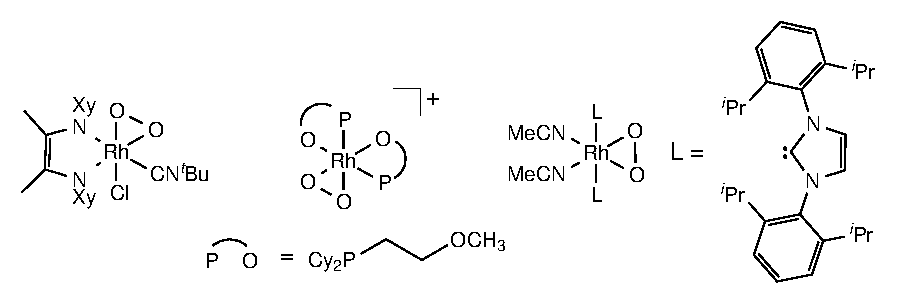
\includegraphics{../Figures/OtherRhO2complexes.eps}
\caption[Rhodium dioxygen complexes with shorter Rh-O bonds than \texorpdfstring{[Rh(\tBuxantphos)(\hapto{2}-\ce{O2})Cl{]}} R]{Rhodium dioxygen complexes with shorter Rh-O bonds than \texorpdfstring{[Rh(\tBuxantphos)Cl(\hapto{2}-\ce{O2}){]}} R.}
\vspace{0.2cm}
\label{ShorterRhOcomplexes}
\end{center}
\end{figure}
\vspace{0.2cm}

The [Rh(\tBuxantphos)Cl(\hapto{2}-\ce{O2)}] complexes, with \tBusixantphos{} or \tBuxantphos{}, show two distinct methyl environments in the \proton{} and \carbon{} NMR spectra for the bridgehead methyls.  This indicates a loss of symmetry, giving two distinct faces of the \tBuxantphos{} ligands.  From the crystal structure (Figure \ref{Crystal:rhodium}) the chloride ligand sits on the same side as the concave face of the ligand while the dioxygen ligand occupies the position pseudo-\emph{trans} to the oxygen bridge of the ligand.  This geometry leaves more space \emph{trans} to the chloride, resulting in the curvature of the ligand to occupy this free space and the tipping of the methyl groups away from the chloride.  The angle O1-C(bridge)-\ce{CH3} is very different for the two methyl groups; 165.9(3) and 94.7(3)\degrees{} for the concave and convex methyls, respectively and dihedral angles to the first C-H in the aromatic ring of 24.8 and 42.8\degrees.  This positioning results in quite different chemical environments for the two methyl groups, resulting in the different chemical shifts in the NMR spectra.  

%Discussion of xantphos dioxygen complexes.
Although rhodium xantphos{} complexes are well studied due to their high catalytic activity and selectivity for hydroformylation, to the best of our knowledge, no rhodium dioxygen complexes have been reported with any xantphos ligands.  Only one transition metal complex with a xantphos related ligand and an \hapto{2} dioxygen ligand has been reported; [Ru(\Phxantphos)\ce{(PPh3})(\hapto{2}-\ce{O2)H]BAr4^F}.\cite{Ledger2010}  This complex formed by reaction of [Ru(\Phxantphos)\ce{(PPh3)HCl]} with \ce{NaBAr4^F} followed by filtration then stirring in the air for 10 minutes.  Similarly to the rhodium \tBuxantphos{} complexes, the \emph{mer}-\POP{} coordination is retained upon reaction with oxygen.  The dioxygen ligand occupies the site \trans{} to the hydride, where the chloride had previously been located.  

The X-ray crystal structure of [Rh(\tBuxantphos)Cl(\hapto{2}-\ce{O2})] contains substitutional disorder with approximately 15\%{} of the dioxygen molecules replaced by an oxo group (Figure \ref{Crystal:rhodiumoxo}).  The oxo complex shows a slightly distorted square-based pyramid structure with the ether bridge of the \tBuxantphos{} ligand occupying the apex, and \trans{} coordination of the phosphorus atoms.  The rhodium oxo bond (1.669(10) \A) is much shorter than the rhodium oxygen bond lengths in [Rh(\tBuxantphos)Cl(\hapto{2}-\ce{O2})], consistent with a higher bond order.  In addition, the rhodium oxo bond is the shortest crystallographically determined Rh-O bond.  

To the best of our knowledge, this is the first example of crystallographic evidence for a rhodium(III) oxo complex. Only one previous crystal structure has been reported for a rhodium oxo complex (Figure \ref{Kaczul}).\cite{Gangopadhyay2010}  The literature structure contains a rhodium(V) dimer with each rhodium atom coordinated to two oxo ligands, a DMSO ligand and an oxygen-nitrogen-sulfur heterotridentate ligand.  The oxo \trans{} to the DMSO ligand has a bond length of 1.701(5) \A, while the oxo \trans{} to the nitrogen donor is slightly longer at 1.712(5) \A.  Both of these are slightly longer than the Rh-O bond length in the [Rh(\tBuxantphos)Cl(O)] structure (1.669(10) \A).  The average bond length for a transition metal oxo is 1.689 \A{} with a lower quartile at 1.671 \A.\cite{Allen2002}  This indicates that the bond length for the rhodium(III) oxo is in the lowest quarter of crystallographically determined bond lengths for transition metal oxo complexes; however, the bond is well within the range (1.106--2.956 \A).  

\begin{figure}[htb]
\begin{center}
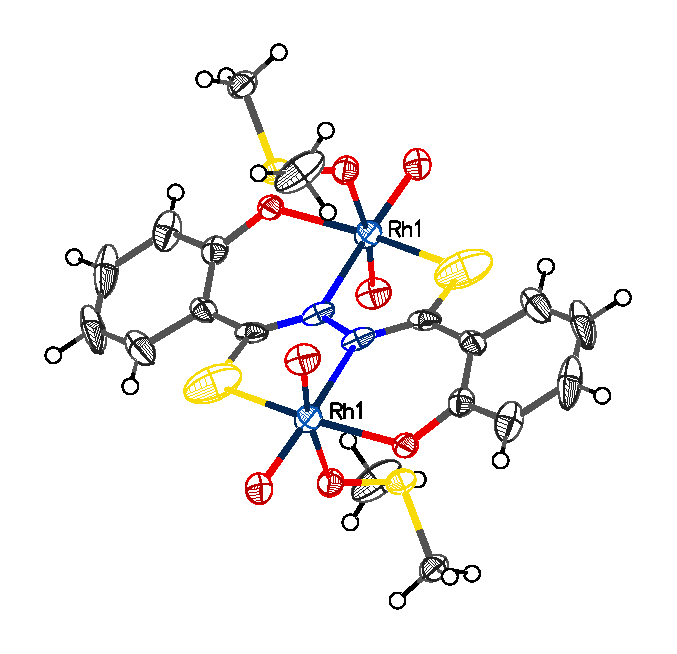
\includegraphics[scale=0.8]{../Othercrystals/KACZUL2.eps}
\caption[A rhodium oxo crystal structure]{An X-ray crystal structure for the rhodium(V) oxo complex \ce{[(RhO2)2(C6H4(O)-C(=S)-N=N-C(=S)(O)C6H4)(DMSO)2]}.\cite{Gangopadhyay2010} Hydrogen atoms omitted for clarity.}
\vspace{0.2cm}
\label{Kaczul}
\end{center}
\end{figure}
\vspace{0.2cm}

Transition metal oxo complexes have long been studied as they have been implicated to have roles in  biological systems,\cite{Lipscomb1994, Merkx2001, Tinberg2011, Montellano2010} C-H activation\cite{Balcells2010, Borovik2011} and various oxidation reactions\cite{Holm1987, Atlay1983, Poverenov2008}.  A terminal oxo ligand is a very strong $\pi$-donor ligand, thus the strongest coordination occurs with high oxidation state, early transition metals\cite{Anderson2004}.  A review of transition metal oxo complexes published in 1987 stated that ``M=O groups are stabilised at metal centres with an oxidation state of no less than +4 and no more than four d electrons''.\cite{Holm1987}  This has led to the proposition of an "oxo-wall," a barrier between groups 8 and 9 of the periodic table, explaining the lack of tetragonal oxo complexes for group 9--11 transition metals.\cite{Winkler2011}  This effect arises as the orbital splitting in an octahedral oxo complex lowers the symmetry of the t\sub{2g} orbitals to b\sub{2}(d\sub{xy}) and e(d\sub{xz},d\sub{yz}) and the metal-ligand anti-bonding e\sub{g} orbitals to b\sub{1}(d\sub{x\superscript{2}-y\superscript{2}}) and a\sub{1}(d\sub{z\superscript{2}}).  with the e(d\sub{xx},d\sub{yz}) and d\sub{z\superscript{2}}, orbitals destabilised.\cite{Betley2008}  The more d-electrons that are present, the lower the bond order to the oxo, resulting in decreased stability.  The [Rh(\tBuxantphos)Cl(O)] complex is of square pyramidal geometry so does not violate the oxo-wall proposition.  The poor electron donation from the central ether bridge may lead to increased stability compared to other square pyramidal structures.  

Despite the instability of terminal oxo complexes of the late transition metals, some examples do exist (Figure \ref{Rhodiumotheroxo}).  A platinum(II) complex with a PCN pincer ligand was reacted with a freshly prepared acetone solution of dioxirane, resulting in formation of a platinum(IV) oxo complex.\cite{Poverenov2008}  This complex degrades over a period of 7--10 hours \emph{via} an intramolecular oxygen transfer reaction from the platinum to the phosphorus atom.  The oxo also readily reacts with water (forming a bishydroxy, aquo complex), hydrogen (liberating water), carbon monoxide (forming \ce{CO2} and a carbonyl complex), potassium hydride (to form a hydroxy complex) and oxidises triphenyl phosphine.  This demonstrates a range of different potential uses for late transition metal oxo complexes.  An iridium(V) oxo complex has also been reported, in this case the oxo complex was synthesised by reaction of \ce{[Ir(mes)3]} (mes = mesityl) with trimethylamine oxide (Figure \ref{Rhodiumotheroxo}).\cite{Motherwell1993}  A rhodium(I) oxo complex was recently reported by Caulton \emph{et al.} from reaction of rhodium(III) hydride complex containing a metalled PNP ligand reacting with trimethylamine oxide, pyridine \emph{N}-oxide or \ce{N2O}.\cite{Verat2008, Tsvetkov2013}  This complex undergoes oxo transfer reactions with trimethylphosphine and carbon monoxide.

\begin{figure}[htb]
\begin{center}
\vspace{0.5cm}
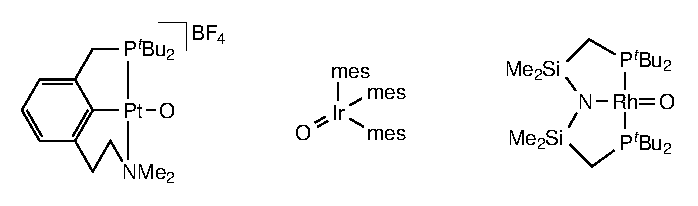
\includegraphics{../Figures/Rhodiumotheroxo.eps}
\caption[Previously reported late transition metal oxo complexes]{Previously reported late transition metal oxo complexes, mes = 2,4,6-trimethylphenyl.\cite{Poverenov2008, Verat2008, Tsvetkov2013}}
\vspace{0.2cm}
\label{Rhodiumotheroxo}
\end{center}
\end{figure}
\vspace{0.2cm}

Given the novelty of a rhodium(III) oxo complex, the synthesis of [Rh(\tBuxantphos)Cl(O)] complexes with all three \tBuxantphos{} ligands was attempted using trimethylamine oxide, as this has been used previously in the synthesis of late transition metal oxo complexes,\cite{Motherwell1993, Tsvetkov2013} and the by-product (trimethylamine) should be a poor ligand and result in little reactivity.    Reaction between [Rh(\tBusixantphos)Cl] and trimethylamine oxide resulted in the immediate formation of the [Rh(\tBusixantphos)Cl(\hapto{2}-\ce{O2})] complex, together with a small amount of the ligand oxide and uncoordinated \tBusixantphos, over time peaks due to the [Rh(\tBusixantphos)Cl] complex began to reappear.  This result may be due to the incomplete dissolution of [Rh(\tBusixantphos)Cl] in the \ce{CD2Cl2} reaction solvent, meaning that the amount in solution was over-oxidised before the remainder dissolved.  Unfortunately, as [Rh(\tBusixantphosk)Cl] is a dark brown colour it is challenging to gauge full dissolution.  After four days at room temperature a small amount of product was evident in the \phosphorus{} NMR spectrum at 70.5 ppm (\JRhP{} = 114.1 Hz).  

Reacting [Rh(\tButhixantphosk)Cl] and trimethylamine oxide resulted in a mixture of compounds.  Analysis by \phosphorus{} NMR showed 22.9\%{} free \tButhixantphos{} ligand indicating possible degradation of the rhodium complexes formed, [Rh(\tBusixantphosk)Cl(\hapto{2}\ce{O2})] (8.6\%{}), [Rh(\tButhixantphosk)Cl] starting material (64.4\%), and a new complex at 40.9 ppm (\JRhP{} = 90.4 Hz) (4.1\%).  After 10 days no [Rh(\tButhixantphosk)Cl] or unidentified complex remained and the reaction mixture was primarily the dioxygen complex and a further new complex at 74.1 ppm (\JRhP{} = 116.3 Hz).  

The reaction of [Rh(\tBuxantphosk)Cl] with trimethylamine oxide was initially carried out at -80 \degC{} in order to prevent over-oxidation.  However, initially the slow generation of the dioxygen species was observed with no evidence for any intermediate or otherwise.  The reaction was allowed to warm to room temperature and after 24 hours a small amount (4.2\%) of a complex at 42.6 ppm (\JRhP{} = 90.4 Hz).  However, around 70.5\%{} of the reaction mixture was the dioxygen complex and the remainder was the Rh(I) starting material.  Similarly to the \tButhixantphos{} reaction, this reaction slowly converted into a species at 75.1 ppm (\JRhP{} = 116.3 Hz).  

The initial unknown complexes formed by the oxidation of [Rh(\tBuxantphosk)Cl] and [Rh(\tButhixantphosk)Cl] had similar NMR spectra. In the \phosphorus{} NMR spectra a doublet was observed at 40.9 or 42.6 ppm, slightly downfield of the dioxygen complex.  The values of \JRhP{} were identical with either ligand (90.4 Hz).  The decrease from the values in the rhodium(I) starting materials (142.3 and 140.0 Hz for \tBuxantphos{} and \tButhixantphos{} respectively) clearly indicates oxidation to a rhodium(III) species.  Mass spectrometry was performed on the reaction mixtures for all three \tBuxantphos{} ligands.  In all cases a molecular ion peak was observed consistent in both mass$/$charge ratio and isotopic pattern, indicative of an oxo complex ionising \emph{via} loss of a chloride ligand.

%Phosphine ligands can act as $\pi$-acceptor ligands with back-donation into P-C $\sigma^*$ bonds which have $\pi$ symmetry.  While the bonding of \tBu{} phosphines is generally dominated by $\sigma$-donation, the \tBuxantphos{} ligands also have an aromatic substituent which enhances the back-bonding relative to trialkylphosphines.  Terminal oxo ligands are strong $\pi$-donor ligands\cite{Betley2008} so we would expect that coordination of an oxo ligand would increase the electron density on the metal, thereby increasing the back-donation to the phosphorus atoms.  This would result in a longer P-M bond and thus lower Rh-P coupling constants are observed in the oxo complexes than in the dioxygen or dihydrogen complexes.  Hence, based on the data discussed we tentatively postulate the identity of the first unknown complex as a square pyramidal rhodium(III) oxo complex (Scheme \ref{Rhodiumoxo}).

\begin{scheme}[htb]
\begin{center}
\vspace{0.5cm}
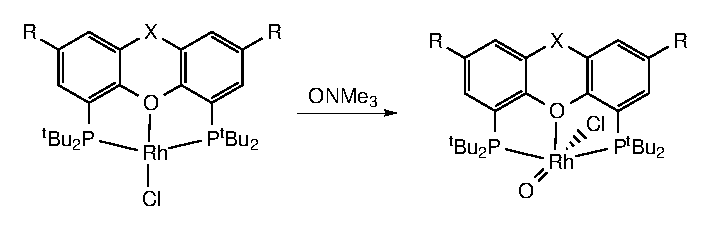
\includegraphics{../Schemes/Rhodiumoxo.eps}
\caption[Reaction of \texorpdfstring{[Rh(\tBuxantphos)Cl{]}} R with trimethylamine oxide]{Reaction of \texorpdfstring{[Rh(\tBuxantphos)Cl{]}} R with trimethylamine oxide. \emph{Reagents and conditions:} 1eq. \ce{ONMe3}, \ce{CD2Cl2}.}
\vspace{0.2cm}
\label{Rhodiumoxo}
\end{center}
\end{scheme}
\vspace{0.2cm}

Late transition metal oxo complexes are generally considered unstable and likely to undergo further reaction.  The reactions of [Rh(\tBuxantphosk)Cl] with trimethylamine oxide were performed in \ce{CD2Cl2}.  As previously discussed (see Section \ref{section:ligands:basicity}) halocarbon molecules are not stable for extended periods of time in the light, undergoing a photo-catalysed degradation forming small amounts of hydrochloric acid (deuterium chloride in the case of NMR solvents).\cite{Yano1977}  Hereby we propose that the oxo complex likely reacted with the small amounts of deuterium chloride that formed over time, thus producing a hydroxy ligand (Scheme \ref{Rhodiumhydroxy}).  The remaining coordination site on the metal would then likely be occupied by the chloride ion.  The platinum oxo complex reported by Milstein \emph{et al.} underwent reaction with water to form a bishydroxy complex while the rhodium oxo reported by Caulton \emph{et al.} underwent metallation of one of the \tBu{} substituents on the phosphorus donor also forming a hydroxy ligand.\cite{Verat2008}  

\begin{scheme}[htb]
\begin{center}
\vspace{0.5cm}
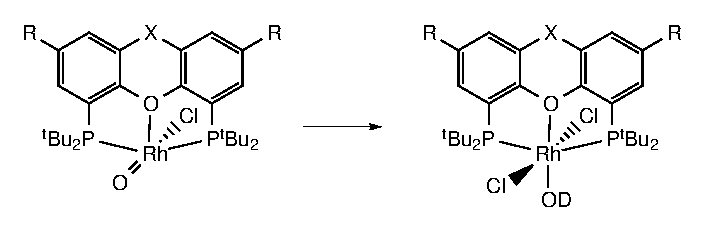
\includegraphics{../Schemes/Rhodiumhydroxy.eps}
\caption[Reaction of \texorpdfstring{[Rh(\tBuxantphos)Cl(O){]}} R with DCl]{Proposed reaction of \texorpdfstring{[Rh(\tBuxantphos)Cl(O){]}} R with DCl.}
\vspace{0.2cm}
\label{Rhodiumhydroxy}
\end{center}
\end{scheme}
\vspace{0.2cm}

Unfortunately, due to time constraints, the formation of the rhodium oxo complexes was not studied in more depth.  

\section{Conclusion}

The coordination chemistry of \tBusixantphos{}, \tButhixantphos{}, and \tBuxantphos{} with rhodium in both the +1 and +3 oxidation states was explored.  The three ligands reacted readily with [Rh(coe\ce{)2Cl]2} forming [Rh(\tBuxantphosk)Cl] complexes.  These complexes readily split hydrogen to form  [Rh(\tBuxantphosk)Cl\ce{(H)2}] complexes with a meridional \tBuxantphos{} ligand and \cis{} hydrides.  Little difference in the position and coupling constants of the hydride \trans{} to the chloride was observed in the \proton{} NMR spectra of the three complexes.  The values of \JRhH{} for the hydride \trans{} to the oxygen donor decreased with increasing bite-angle.  Suggesting a \trans{} influence series of \tBuxantphos{} \textgreater{} \tButhixantphos{} \textgreater{} \tBusixantphos{}.  This difference may be related to the ease with which the ligands form wide bite-angle complexes.

The three [Rh(\tBuxantphosk)Cl] complexes were reactive towards carbon monoxide, forming [Rh(\tBuxantphos\dento{}-\emph{P,P}\textprime{})(CO\ce{)2}Cl]. In contrast, \Phxantphos{} and DPEphos{} formed \trans-[Rh(CO)Cl(diphosphine)] complexes.  The \tBuxantphos{} ligands were coordinated in a \dento{}-\emph{P,P}\textprime{} bisequatorial mode with an equatorial chloride and two axial carbonyl ligands.  This shows a clear difference in the reactivity of the \tBuxantphos{} ligands when compared with \Phxantphos.

The rhodium dioxygen complexes, [Rh(\tBuxantphos)Cl(\hapto{2}-\ce{O2})] with the \tBuxantphos{} ligands were synthesised by reaction of  [Rh(\tBuxantphosk)Cl] with the air.  These are the first rhodium dioxygen complexes with xantphos ligands and only the second with any transition-metals.  The X-ray crystal structure of [Rh(\tBuxantphos)Cl(\hapto{2}-\ce{O2})] was reported showing a distorted octahedral configuration with a meridional coordination of the \tBuxantphos{} ligand.  The O-O bond length was typical for rhodium dioxygen complexes.  The Rh-O bond length for the oxygen \trans{} to the oxygen donor of the \tBuxantphos{} ligand was the fourth shortest Rh-O length for a dioxygen complex that have been reported, indicating the low \trans-influence of the \tBuxantphos{} oxygen.  

The X-ray crystal structure of [Rh(\tBuxantphos)Cl(\hapto{2}-\ce{O2})] was disordered with the dioxygen ligand replaced in around 15\% of sites by an oxo ligand.  To the best of our knowledge this is the first crystallographic evidence of a rhodium(III) oxo complex.  The Rh-O bond length was 1.669(10) \si{\angstrom} which is the shortest reported rhodium oxo bond length.  The complex is a distorted square pyramid, so does not violate the ``oxo-wall'' theory.  Attempts to synthesise [Rh(\tBuxantphosk)Cl(O)] by reaction of [Rh(\tBuxantphosk)Cl] with trimethylamine oxide were promising for \tButhixantphos{} and \tBuxantphos{}, showing a new peak in the \phosphorus{} NMR spectra, which slowly converted into a different species, and mass spectra consistent with [Rh(\tBuxantphosk)(O)\ce{]+}.  Future work is required to characterise these species.  

Overall, a number of new rhodium complexes were synthesised including the \tBuxantphos{} ligands in \POP{} square planar and trigonal bipyramidal complexes, and \dento{}-\emph{P,P}\textprime{} coordination modes in trigonal bipyramidal geometries.  

%\section{Iridium Complexes}
%\label{section:experimental:iridium}

%Reaction between \ce{[Ir(COE)2Cl]2} and iPr-xantphos resulted in an iridium(III) complex with the iPr-xantphos coordinating tetradentate through the phosphines, oxygen and a metalled methyl of an isopropyl group.\cite{Esteruelas2013}  Also coordinated are the original chloride ligand and a hydride formed in the metallation.  The reaction likely proceeds via a \ce{[Ir($\eta^3-$iPr-xantphos)Cl]} and then metallation occurs.  However, no spectroscopic evidence for the \ce{Ir($\eta^3-$iPr-xantphos)Cl]} was reported.  Given that metallation occurs on platinum for the reaction between the dioxygen complex and carbon monoxide \fixme{reference} it was expected that metallation should occur in a relatively facile manner when the tBu-xantphos ligands were reacted with \ce{[Ir(COE)2Cl]2}.  

%However, when the reactions were carried out they proved to be very slow, and gave intractable mixtures of products.  In each case a large number of hydride resonances were observed indicating that metallation had occurred however, the nature of the complexes was unable to be determined.  The reactions became dark relatively rapidly though they continued to react after this colour change was observed.  The \ce{[Rh($\eta^3-$tBu-xantphos)Cl]} complex was dark red so the colour change is not necessarily a sign of degradation of the iridium starting material.  














